\documentclass[12pt,a4paper]{article}
\usepackage[utf8]{inputenc}
\usepackage[german]{babel}
\usepackage[T1]{fontenc}
\usepackage{amsmath}
\usepackage{amsfonts}
\usepackage{amssymb}
\usepackage{graphicx}
\usepackage{float}
\usepackage[left=2cm,right=2cm,top=2cm,bottom=2cm]{geometry}
\author{Tim}

\begin{document}

\tableofcontents
\newpage

\section{Charakterisierung Ohm'scher Widerstand}
\subsection{Versuchsbeschreibung}
Es soll der in den nachfolgenden Versuchen verwendete Ohm'sche Widerstand charakterisiert werden. Dazu wird der Widerstand in einen Gleichstromkreis mit einer Spannungsquelle und einem Strommessgerät eingebaut. Nach dem Ohm'schen Gesetz gilt dann:
\begin{equation}
R = \dfrac{U}{I}
\label{eq:Ohm}
\end{equation}
\subsection{Aufbau und Durchführung}
\begin{figure}
\begin{center}
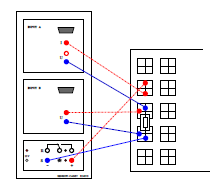
\includegraphics[scale=1.2]{Bilder/Charakterisierung_Widerstand_Aufbau.PNG}
\end{center}
\caption[Widerstand Schaltung]{Aufbau für die Charakterisierung des Widerstands}
\label{fig:Widerstand_Aufbau}
\end{figure}
Abbildung \ref{fig:Widerstand_Aufbau} zeigt den Aufbau. Es wird ein Stromkreis aus Spannungsquelle, Strommessgerät, Widerstand und Spannungsmessgerät über den Widerstand aufgebaut.\\
\\ Die Spannungsquelle wird auf einen Wert eingestellt und die Messung gestartet. Dabei werden viele Werte für Strom und Spannung aufgezeichnet. Die verwendeten CASSY-Einstellungen sind:\\
\begin{center}
\begin{tabular}{|c|c|}

\hline 
Intervall & $10 \mu s$ \\ 
\hline 
Anzahl Messwerte pro Messreihe & 4000 \\ 
\hline 
Messbereich I & $|I| \leq 0,3A$ \\ 
\hline 
Messbereich U & $|U| \leq 10A$ \\ 
\hline 

\end{tabular} 
\end{center}
\subsection{Auswertung}
\subsubsection{Rauschmessungen}
Die Mehrfachmessungen bei gleichem Aufbau können zusätzlich auch als Rauschmessung für die Spannung und den Strom verwendet werden. Dazu wird für jede eingestellte Spannung die Standardabweichung aus der Mehrfachmessung bestimmt. Die Standardabweichungen finden sich in folgender Tabelle: \\
\begin{center}
\begin{tabular}{|c|c|c|}
\hline 
Messung & Standardabweichung auf Strom [mA] & Standardabweichung auf Spannung [mV] \\ 
\hline 
1 & 0,08 & 2,3 \\ 
\hline 
2 & 0,08 & 2,5 \\ 
\hline 
3 & 0,10 & 2,4 \\ 
\hline 
4 & 0,09 & 2,8 \\ 
\hline 
5 & 0,11 & 2,7 \\ 
\hline 
6 & 0,08 & 2,5 \\ 
\hline 
7 & 0,07 & 2,3 \\ 
\hline 
8 & 0,10 & 2,3 \\ 
\hline 
9 & 0,09 & 2,7 \\ 
\hline 
\end{tabular}
\end{center}
In den nachfolgenden Versuchen wurde, um nur einen Wert für den Fehler auf Strom und Spannung zu haben und trotzdem alle Messungen zu berücksichtigen, der Mittelwert der Standardabweichungen aus den neun Messungen verwendet:
\[\sigma_U = 2,48 mV \quad und \quad \sigma_I = 0,088 mA \]


\subsubsection{Lineare Regression und Statistischer Fehler}
Stellt man Gleichung \ref{eq:Ohm} um, erhält man folgenden Ausdruck:
\begin{equation}
U = R \cdot I
\end{equation}
Daran lässt sich direkt ersehen, dass sich bei Auftragung des Stroms auf die X-Achse und der Spannung auf die Y-Achse der Widerstand als Steigung der Geraden ergibt. Da auf den Achsen direkt die gemessenen Größen aufgetragen werden können, wird die lineare Regression direkt auf die Rohdaten angewandt. \\
Aus den Messungen von Strom und Spannung für jede eingestellte Spannung kann jeweils Mittelwert und Standardabweichung bestimmt werden. Abbildung \ref{fig:Widerstand_lineare_Regression} zeigt die Rohdaten als blaue Punkte mit Fehlerbalken und das Ergebnis der lineare Regression als rote Gerade. Die negative Steigung der Geraden ist bedingt durch das negative Vorzeichen des Stroms und das liegt lediglich an der Polung des Messgerätes. Für den realen Wert des Widerstandes muss der Betrag der Steigung genommen werden; am Fehler ändert sich nichts. \\
Die linearen Regressionen ergeben ein sehr kleines $\chi^2$ pro Freiheitsgrad (siehe beispielsweise Abbildung \ref{fig:Widerstand_lineare_Regression}). Dies bedeutet, dass die Fehler zu groß sind. Vermutlich liegt das an dem anfangs verwendeten CASSY. Dieses zeigte zum Teil extrem schwankende und dabei (für kurze Zeiten) physikalisch unsinnige Werte an. Das CASSY wurde nach der Charakterisierung des 100 $\Omega$ Widerstands ausgewechselt. Aus Zeitgründen konnten die mit dem ersten (scheinbar kaputten) CASSY durchgeführten Messungen nicht wiederholt werden. Da die falschen Werte immer nur für eine kurze Zeit angezeigt wurden, stimmt der Wert im Mittel über viele in der Zeit gleichverteilte Werte wieder (wie sich am Ergebnis auch zeigen wird), daher kann die Messung dennoch verwendet werden.
\begin{figure}
\begin{center}
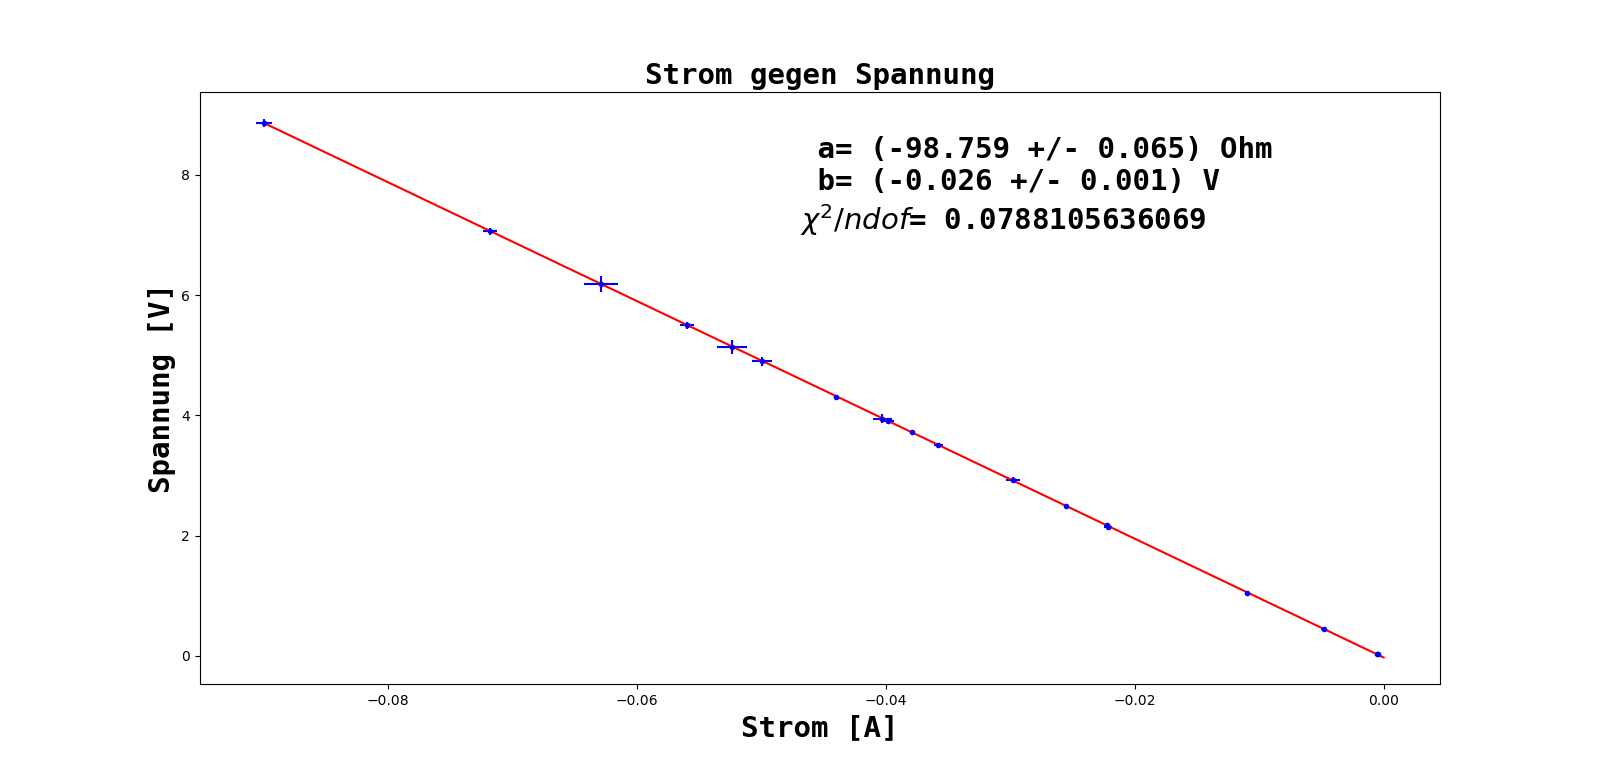
\includegraphics[scale=0.45]{Bilder/Widerstand_Fit.png}
\end{center}
\caption[Widerstand Lineare Regression]{Lineare Regression an Strom und Spannung}
\label{fig:Widerstand_lineare_Regression}
\end{figure}
\subsubsection{Systematischer Fehler}
Um den Einfluss der Systematik auf den Widerstand zu erhalten, wird die sogenannte Verschiebemethode angewandt. Dabei werden Strom und Spannung jeweils um den systematischen Fehler einmal nach oben und einmal nach unten verschoben und die lineare Regression erneut durchgeführt. Dabei werden die Spannung und der Strom jeweils um den vom Hersteller angegebenen systematischen Fehler verschoben:
\begin{equation}
U_{i, verschoben} = U_i \pm (0,01 \cdot U_i + 0,005 \cdot U_{Bereichsendwert})
\end{equation}
\begin{equation}
I_{i, verschoben} = I_i \pm (0,02 \cdot I_i + 0,005 \cdot I_{Bereichsendwert})
\end{equation}
Der systematische Fehler auf den Widerstand berechnet sich dann zu:
\begin{equation}
\Delta R_{sys}^2 = \left(\dfrac{|R_{U,-}-R| + |R_{U,+}-R|}{2}\right)^2 + \left(\dfrac{|R_{I,-}-R| + |R_{I,+}-R|}{2}\right)^2
\end{equation}
Die Endergebnisse, die Messergebnisse von der Brücke und dem Multimeter sowie die Herstellerangaben für die Widerstände finden sich in folgender Tabelle:\\
\begin{tabular}{|c|c|c|c|}
\hline 
Herstellerangabe [$\Omega$] & Multimeter [$\Omega$] & Brücke [$\Omega$] & lineare Regression [$\Omega$] \\ 
\hline 
10 $\pm$ 0,5 & 10,1 $\pm$ 0,03 $\pm$ 0,58 & 9,98 $\pm$ 0,02 $\pm$ 0,01 & 9,94 $\pm$ 0,01 $\pm$ 0,22 \\ 
\hline 
100 $\pm$ 5 & 99,4 $\pm$ 0,03 $\pm$ 1,30 & 99,4 $\pm$ 0,25 $\pm$ 0,10 & 98,74 $\pm$ 0,06 $\pm$ 2,20 \\ 
\hline 
\label{tab:Widerstand_Ergebnisse}
\end{tabular} \\
Es lässt sich gut erkennen, dass die Messwerte aller Messmethoden sehr nah an der Herstellerangabe liegen. Insbesondere liegen alle Messwerte innerhalb der vom Hersteller angegebenen Toleranz.
\newpage
\section{Kondensator}
\subsection{Versuchsbeschreibung}
In diesem Teilversuch soll die Kapazität eines Kondensators durch Auf- und Entladung von diesem bestimmt werden.
\subsubsection{Aufladung}
Wird eine Spannung an einen Kondensator angelegt, so wird dieser geladen, bis die Quellspannung kompensiert wird. Der Ladevorgang dauert umso länger, je größer der Widerstand des Stromkreises ist.\\
Aus der Maschenregel folgt:
\begin{equation}
U_0 = U_R + U_C \Rightarrow U_0 - U_C = R\cdot C\cdot \dfrac{dU_c}{dt}
\label{Kondensator_DGL}
\end{equation}
Bei der Aufladung kann man daraus den Strom und die Spannung bestimmen:
\begin{equation}
U_C(t) = U_0 \cdot (1-e^{-\dfrac{t}{R\cdot C}})
\end{equation}
\begin{equation}
I(t) = I_0 \cdot e^{-\dfrac{t}{R\cdot C}}
\end{equation}
Dabei ist $\tau = R \cdot C$ die Zeitkonstante des R-C-Kreises.
\subsubsection{Entladung}
Bei der Entladung liegt keine externe Spannung mehr an. Es gilt also: $U_0 = 0$\\
Mit dieser Annahme und Gl. \ref{Kondensator_DGL} folgt:
\begin{equation}
U_C(t) = U_0 \cdot e^{-\dfrac{t}{R\cdot C}}
\end{equation}
\begin{equation}
I(t) = -I_0 \cdot e^{-\dfrac{t}{R\cdot C}}
\end{equation}
\subsection{Aufbau und Durchführung}
\begin{figure}[H]
\begin{center}
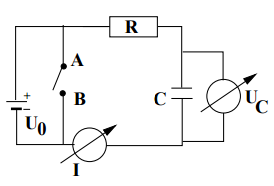
\includegraphics[width=0.75\linewidth]{Bilder/Kondensator_Aufbau}
\caption[Aufbau Kondensator]{Aufbau Kondensator}
\label{fig:Kond_Aufbau}
\end{center}
\end{figure}

\begin{table}[H]
\begin{center}
\begin{tabular}{|c|c|c|}
\hline 
Bauteil & Angegebener Wert & Bestimmter Wert \\ 
\hline 
Widerstand & 100 & $98.74\pm 0.06\pm2.2$ \\ 
\hline 
Kondensator & 4.7 & zu bestimmen \\ 
\hline 
\end{tabular} 
\end{center}
\caption{Angaben zu verwendeten Bauteilen}
\label{tab:Kond_Hersteller} 
\end{table}

Der Versuch wird gemäß Abb. \ref{fig:Kond_Aufbau} aufgebaut. Dabei wird als Spannungsquelle die des CASSY benutzt.Diese wird mit dem Stromkreis, bestehend aus einem Widerstand, einem Kondensator und dem Strommessgerät, verbunden. Um die Entladung des Kondensators durchführen zu können wird noch ein Schalter so eingebaut, dass die Spannungsquelle kurzgeschlossen werden kann.\\ 
Die Bauteileigenschaften  der verwendeten Teile sind in Tabelle \ref{tab:Kond_Hersteller} aufgelistet.
Über Kanal A des CASSY wird der Stromfluss gemessen und über Kanal B die Spannung am Kondensator.\\
Gleichzeitig wird auch Strom und Spannung mit einem Oszilloskop gemessen. Dafür wird an Kanal 2 des Oszilloskopes der Spannungsabfall über den Widerstand und an Kanal 1 die Spannung über den Kondensator angeschlossen. Die Erde wird zwischen Kondensator und Widerstand gelegt.\\
\\
Um den Aufladevorgang zu messen, wird die Spannungsquelle beim Start einer Messung aktiviert.
Beim Entladevorgang bleibt die Spannungsquelle eingeschaltet. Der Messvorgang wird über einen Trigger gestartet, der den Spannungsabfall registriert.
\subsubsection{Messung mit dem Oszilloskop}
Messeinstellungen:
\begin{tabular}{c c c}
Messeinstellungen: & Zeitauflösung: $500\mu s$  & Spannungsauflösung: $0.2V$ \\ 
\end{tabular} 
\\
\\
Die Achsenauflösungen sollten so gewählt werden, dass man die Werte möglichst gut ablesen kann.
Der Trigger sollte an der Spannungskurve anliegen.
\subsubsection{Messung mit CASSY}
\begin{tabular}{c c c c}
Messparameter & Messintervall: $10\mu s$  & Anzahl Messwerte: 1000 & automatische Aufnahme \\ 
Messbereiche & Strom: 0.3A & Spannung: 3V \\
Trigger: 2V & angelegte Spannung: 2.1V\\
\end{tabular} 
\paragraph{Aufladung}
Die Spannungsquelle sollte so eingestellt sein, dass sie sich bei Versuchstart automatisch aktiviert. Durch die zeitgleiche Aktivierung der Quelle und dem Start der Messreihe kann es geschehen, dass die ersten paar Messwerte verfälscht werden.
\paragraph{Entladung}
Hier sollte die Spannungsquelle dauerhaft eingestellt sein. Die Messreihe wird gestartet, sobald der Trigger ausgelöst wird.
\newpage
\subsection{Auswertung Oszilloskop}
Während der Versuchdurchführung wurde bereits mit dem Oszilloskop eine Schnellauswertung durchgeführt.
Um die Kapazität zu bestimmen wurden jeweils bei Auf- und Entladung zwei Zeiten mit dazugehörigen Spannungen aufgenommen. Dabei wurden immer Werte an der Spannungskurve aufgenommen, da die Stromkurve sehr starke Schwankungen hatte und dadurch vermutlich ungenauer gewesen wäre.\\
\begin{table}[H]
\begin{center}
\begin{tabular}{|c|c|c|c|c|c|}
\hline 
 & Offset & t1 & U1 & t2 & U2 \\ 
\hline 
Aufladung & -1.18V & -5.2ms & -0.928V & $0.5ms$ & -0.240V \\ 
\hline 
Entladung & -16mV & $0.34ms$ & -1.18V & $0.98ms$ & -0.08V \\ 
\hline 
\end{tabular} 
\end{center}
\label{tab:Kond_Osz}
\caption{Messdaten mit Oszilloskop}
\end{table}
Die gemessenen Werte sind in Tab\ref{tab:Kond_Osz} aufgeführt. Die Kapazität wird folgendermaßen bestimmt:
\begin{equation}
\dfrac{U1}{U2} = e^{-\dfrac{t1-t2}{R\cdot C}}
\end{equation}
Nach C auflösen ergibt:
\begin{equation}
C = \dfrac{t1-t2}{R\cdot \ln(\dfrac{U1}{U2})}
\end{equation}




Die statistischen Fehler dieser Werte werden durch die Ableseungenauigkeit bestimmt. Dabei gilt:
\begin{equation}
\sigma_t = \dfrac{0.1ms}{\sqrt{12}} = 0.03ms
\end{equation}
\begin{equation}
\sigma_U = \dfrac{0.01V}{\sqrt{12}} = 0.003V
\end{equation}
Es ergeben sich schließlich folgende Werte
\begin{table}[H]
\begin{center}
\begin{tabular}{|c|c|}
\hline 
 & Gemessener Wert \\ 
\hline 
Aufladung & $4.69\pm 0.05\pm 0.08$ \\ 
\hline 
Entladung & $4.88\pm 0.02\pm 0.05$ \\ 
\hline 
\end{tabular} 
\end{center}
\caption{Endergebnisse Oszilloskopmessung}
\end{table}
Die Fehler wurden dabei folgendermaßen bestimmt:
\begin{equation}
\sigma_{Cstat} = \sqrt{2\cdot\left(\dfrac{\sigma_t}{R\cdot ln(\dfrac{U1}{U2})}\right)^{2}+\left(\dfrac{-\sigma_U\cdot(t1-t2)}{R\cdot U1\cdot ln(\dfrac{U1}{U2})^{2}}\right)^{2}+\left(\dfrac{\sigma_U\cdot(t1-t2)}{R\cdot U2\cdot ln(\dfrac{U1}{U2})^{2}}\right)^{2}}
\end{equation}
\begin{equation}
\sigma_{Csys} = \dfrac{(t2-t1)\cdot \sigma_R}{R^{2}\cdot ln(\dfrac{U1}{U2})}
\end{equation}

\subsection{Auswertung CASSY}
Über das CASSY wurden bei Auf- und Entladung jeweils 5 Datensätze aufgenommen.
\subsubsection{Rohdaten}
Die Rohdaten Folgen einem logarithmischem Verlauf. Es ist also sinnvoll, diese zu logarithmieren. Dabei wird die \textbf{Spannung beim Aufladen} mit
\begin{equation}
U_{log} = log(U_0-U)
\end{equation}
geändert. Alle anderen Werte wurden mit
\begin{equation}
U_{log} = log(U)
\end{equation}
\begin{equation}
I_{log} = log(I)
\end{equation}
logarithmiert.\\
In den folgenden Beispielplots erkennt man, dass diese logarithmische Darstellung nur am Anfang des Messbereiches sinnvoll ist, da im späteren die Schwankung zu stark wird und der Verlauf nicht mehr logarithmisch ist.\\
Es wurde immer der Betrag der Messwerte genommen. Deswegen ist der Strom beim Entladen positiv.
\begin{figure}[H]
\begin{center}
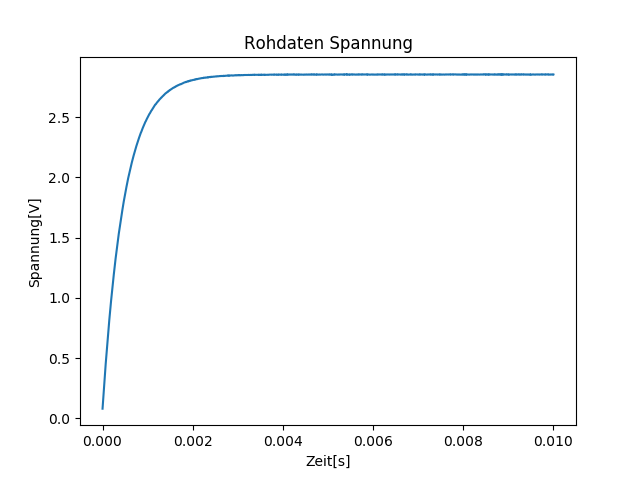
\includegraphics[width=0.49\linewidth]{Bilder/Kondensator_U}
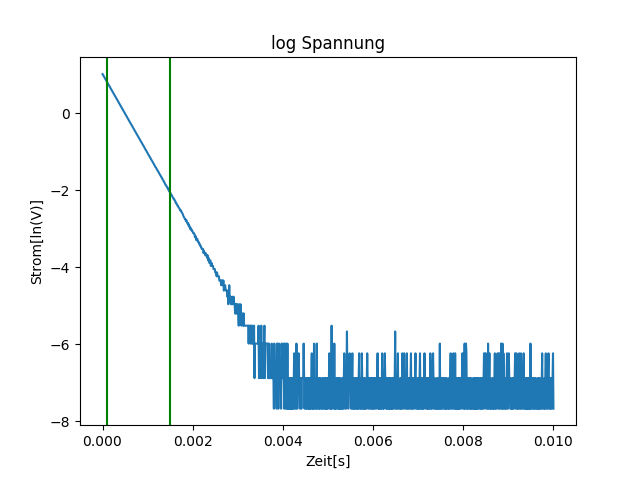
\includegraphics[width=0.49\linewidth]{Bilder/Kondensator_logU}
\caption[Rohdaten logarith. A]{Rohdaten Spannung beim Aufladen}
\label{fig:RohU}
\end{center}
\end{figure}

\begin{figure}[H]
\begin{center}
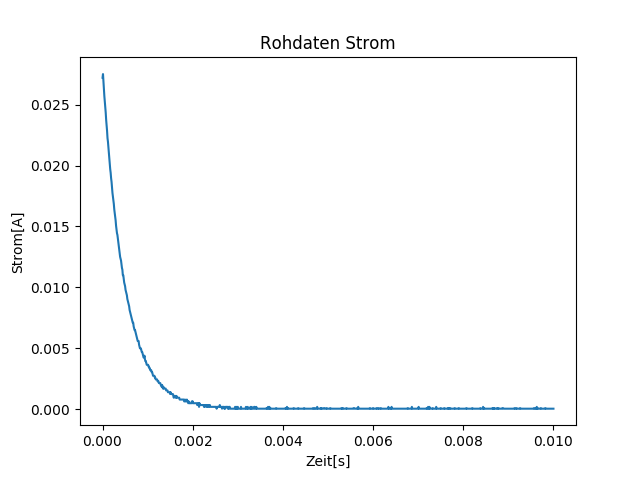
\includegraphics[width=0.49\linewidth]{Bilder/Kondensator_I}
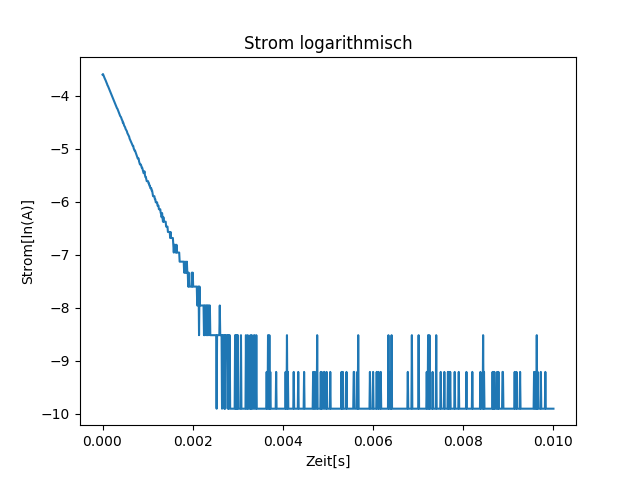
\includegraphics[width=0.49\linewidth]{Bilder/Kondensator_logI}
\caption[Rohdaten logarith. A]{Rohdaten Strom beim Aufladen}
\label{fig:RohU}
\end{center}
\end{figure}

\begin{figure}[H]
\begin{center}
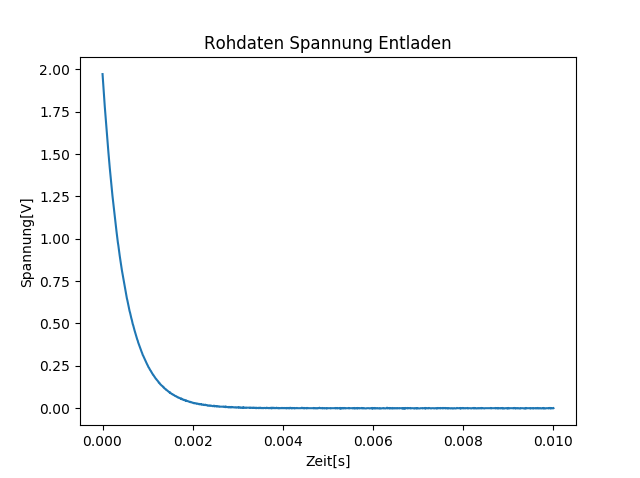
\includegraphics[width=0.49\linewidth]{Bilder/Kondensator_ent_U}
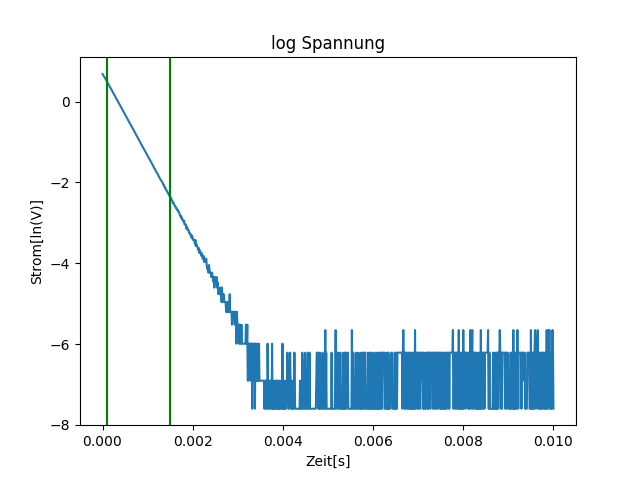
\includegraphics[width=0.49\linewidth]{Bilder/Kondensator_ent_logU}
\caption[Rohdaten logarith. A]{Rohdaten Spannung beim Entladen}
\label{fig:RohU}
\end{center}
\end{figure}

\begin{figure}[H]
\begin{center}
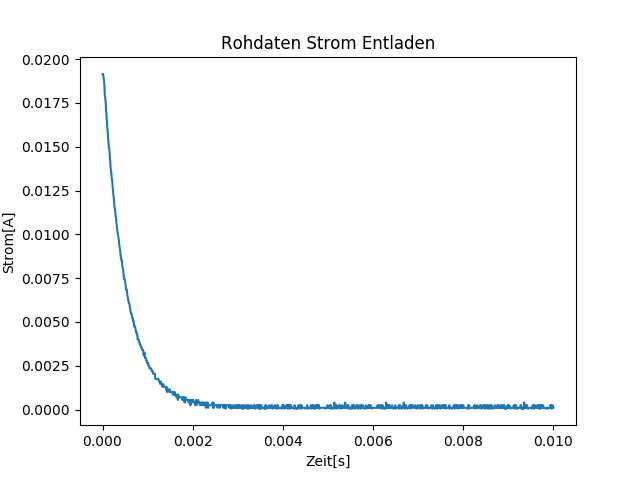
\includegraphics[width=0.49\linewidth]{Bilder/Kondensator_ent_I}
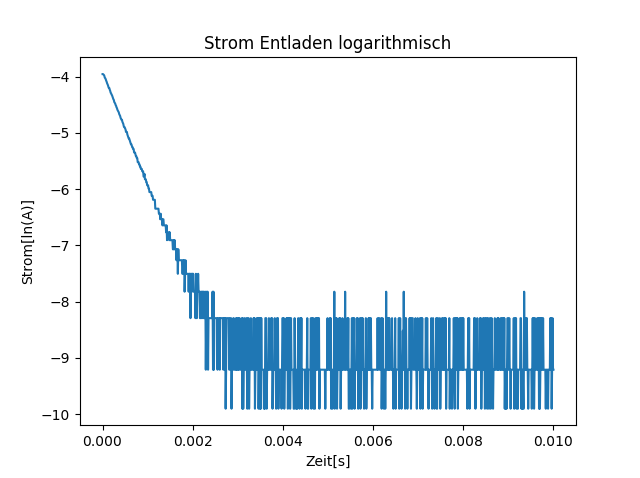
\includegraphics[width=0.49\linewidth]{Bilder/Kondensator_ent_logI}
\caption[Rohdaten logarith. A]{Rohdaten Strom beim Entladen}
\label{fig:RohU}
\end{center}
\end{figure}
\subsubsection{lineare Regressionen}

\begin{figure}
\begin{center}
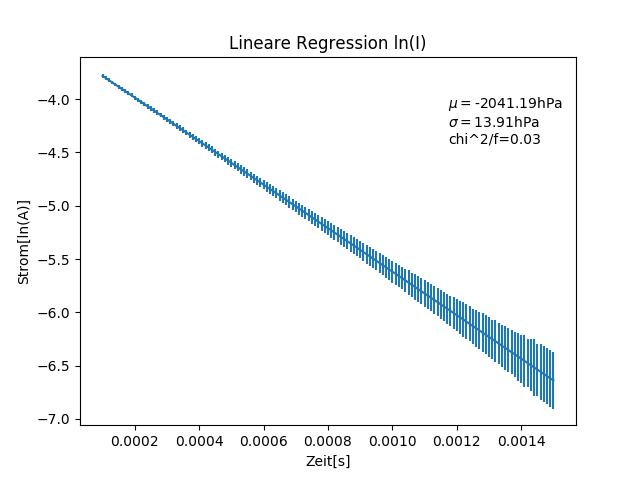
\includegraphics[width=0.49\linewidth]{Bilder/Kondensator_auf_linI}
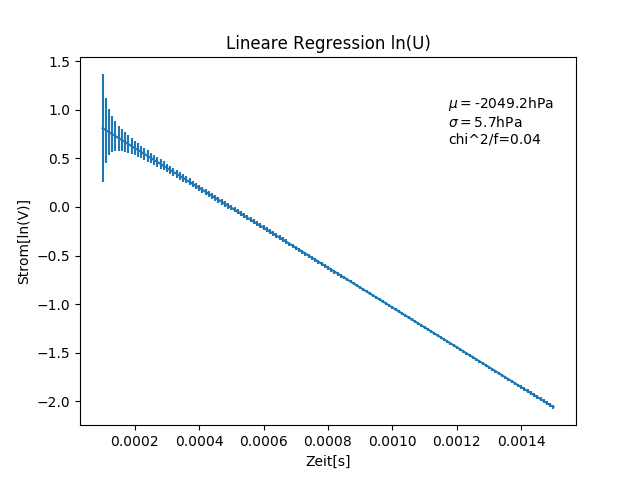
\includegraphics[width=0.49\linewidth]{Bilder/Kondensator_auf_linU}
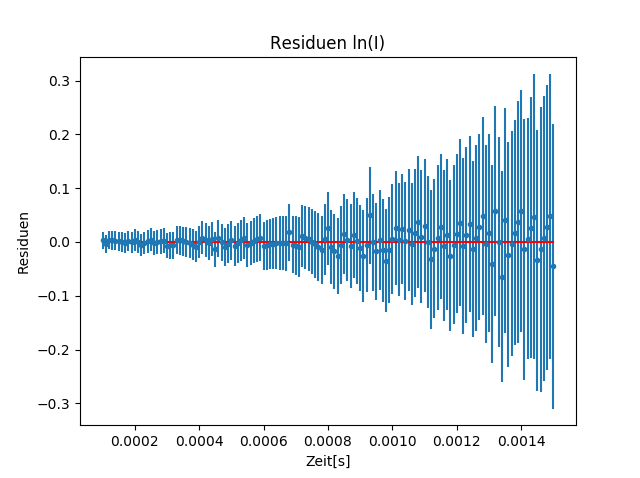
\includegraphics[width=0.49\linewidth]{Bilder/Kondensator_auf_resI}
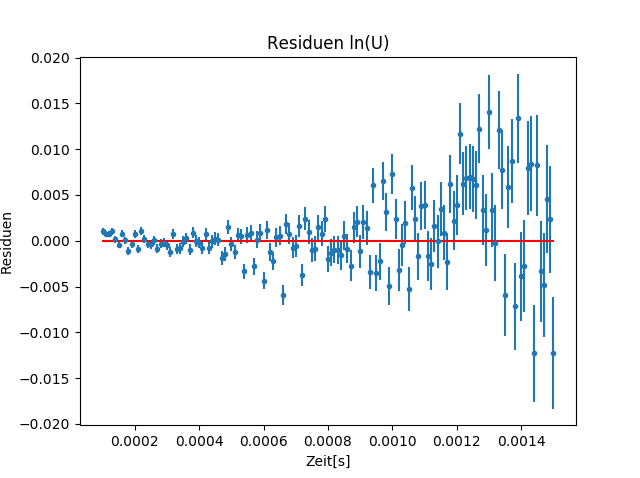
\includegraphics[width=0.49\linewidth]{Bilder/Kondensator_auf_resU}
\caption[Rohdaten logarith. A]{Lineare Regressionen bei der Aufladung(links: Strom, rechts: Spannung}
\label{fig:linAuf}
\end{center}
\end{figure}

\begin{figure}
\begin{center}
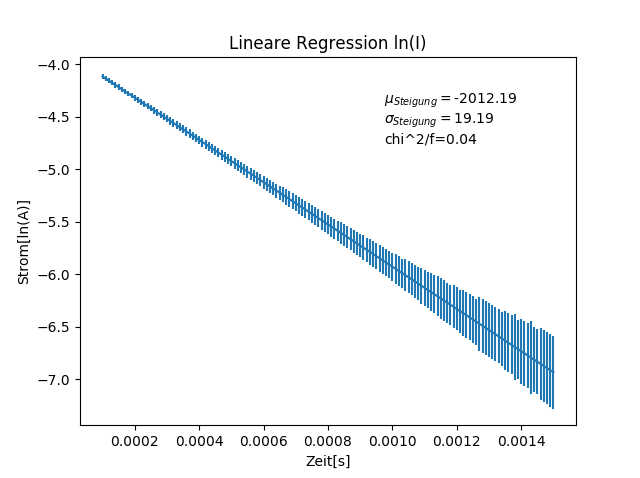
\includegraphics[width=0.49\linewidth]{Bilder/Kondensator_ent_linI}
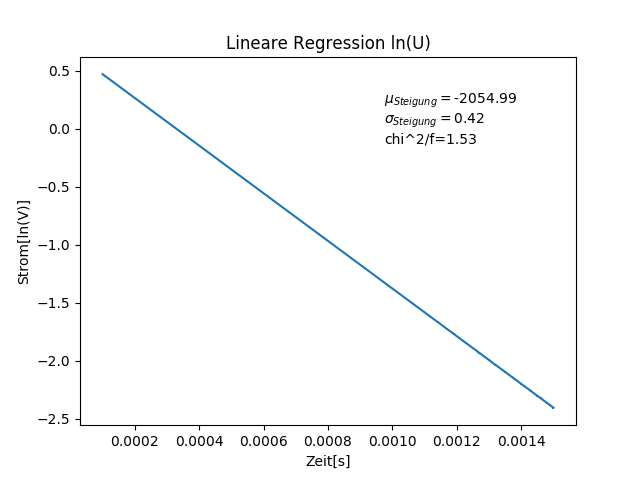
\includegraphics[width=0.49\linewidth]{Bilder/Kondensator_ent_linU}
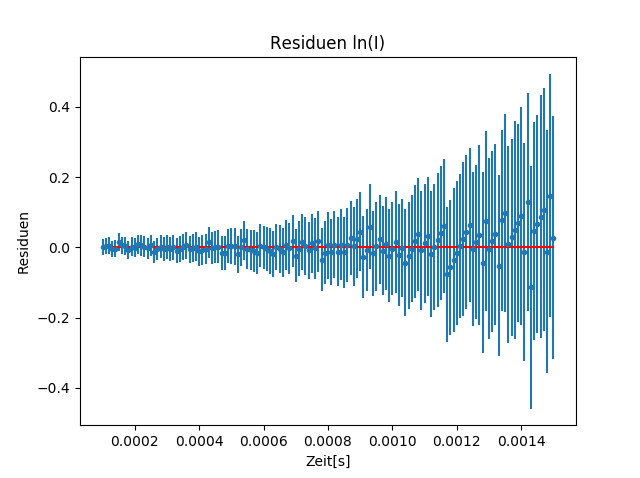
\includegraphics[width=0.49\linewidth]{Bilder/Kondensator_ent_resI}
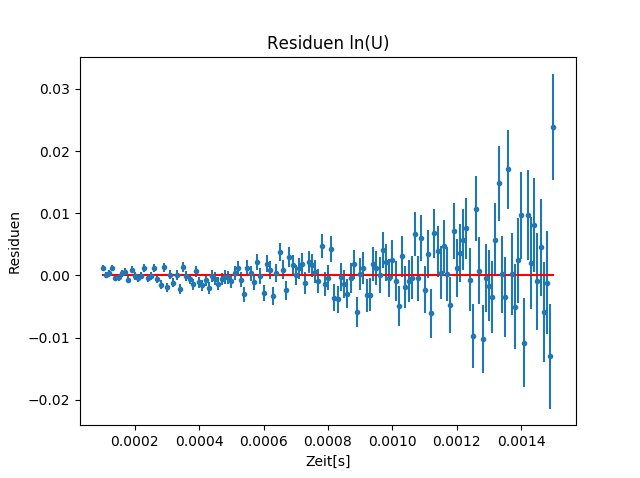
\includegraphics[width=0.49\linewidth]{Bilder/Kondensator_ent_resU}
\caption[Rohdaten logarith. A]{Lineare Regressionen bei der Entladung(links: Strom, rechts: Spannung)}
\label{fig:linEnt}
\end{center}
\end{figure}

Zur Bestimmung der Kapazität wird nun für jeden Datensatz eine lineare Regression an den logarithmisirten Daten durchgeführt. Da die Daten aber zum messende hin von der logarithmischen Darstellung abweichen, wurde nur das Zeitivervall von 0.1ms bis 1.5ms für die Auswertung genommen.\\
In Tab.\ref{tab:kond_linreg} sind dabei jeweils die Mittelwerte der fünf Datensätze für die Auswertung am Strom und an der Spannung aufgelistet.\\
Als Einzelfehler für die lineare Regression wurde der durch Fehlerfortpflanzung errechnete Fehler auf den logarithmisirten Daten verwendet:
\begin{equation}
\sigma_{log(U)} = \dfrac{\sigma_U}{U}
\end{equation}
\begin{equation}
\sigma_{log(I)} = \dfrac{\sigma_I}{I}
\end{equation}
Wobei $\sigma_U$ und $\sigma_I$ den Rauschmessungsfehlern aus dem vorherigen Versuch entsprechen.\\
Anmerkung: Da die Rauschmessung mit dem kapputen CASSY durchgeführt wurde, sind die Fehler vermutlich viel zu groß. Dies resultiert in zu kleinen $\chi ^{2}/f$.

\begin{table}
\begin{tabular}{|c|c|c|c|}
\hline 
 & Steigung & Fehler Steigung & $\chi ^{2}/f$ \\ 
\hline 
Aufladung U & -2049 & 6 & 0.04 \\ 
\hline 
Aufladung I  & -2051 & 14 & 0.03 \\ 
\hline 
Entladung U & -2009 & 20 & 0.03 \\ 
\hline 
Entladung I  & -2028 & 20 & 0.12 \\ 
\hline 
\end{tabular} 
\caption{Mittelergebnisse für die Linearen Regressionen}
\label{tab:kond_linreg} 
\end{table}

\subsubsection{gemessene Daten}
Über die bei der linearen Regression ermittelte Steigung kann man nun durch $\tau = -1/a$ die Zeitkonstante $\tau$ ausrechnen und daraus schließlich mit $C=\dfrac{\tau}{R}$ die Kapazität.
Der Fehler auf $\tau$ ergibt sich dabei folgendermaßen:
\begin{equation}
\sigma_{\tau}=\dfrac{\sigma_{a}}{a^{2}}
\end{equation}
Der statistische Fehler auf C ergibt sich durch
\begin{equation}
\sigma_C = \sqrt{(\dfrac{\sigma_{\tau}}{R})^{2}+(\dfrac{\tau \cdot \sigma_{R}}{R^{2}})^{2}}
\end{equation}
Der systematische Fehler auf C wird aus dem systematischen des Widerstandes fortgepflanzt.
\begin{table}[H]
\begin{tabular}{|c|c|c|}
\hline 
 & Zeitkonstante[$ \mu F\Omega$] & Kapazität[$ \mu F$] \\ 
\hline 
Spannung Aufladung & $0.4880\pm0.0006$ & $4.941\pm0.007\pm0.123$ \\ 
\hline 
Strom Aufladung & $0.4877\pm0.0015$ & $4.938\pm0.015\pm0.123$ \\ 
\hline 
Spannung Entladung & $0.4977\pm0.0022$ & $5.027\pm0.023\pm0.123$ \\ 
\hline 
Strom Entladung & $0.4924\pm0.0022$ & $4.974\pm0.023\pm0.123$ \\ 
\hline 
\end{tabular}
\caption{Ergebnisse für Kapazität und die Zeitkonstante}
\end{table}

Um einen endgültigen Endwert zu bestimmen, werden nun alle Ergebnisse für die Kapazität mit ihrem statistischen Fehler gewichtet gemittelt. Damit erhält man folgendes Endergebnis:
\begin{equation}
C_{ges} = (4.951\pm 0.006\pm0.123)\mu F
\end{equation}

\begin{tabular}{|c|c|}
\hline 
Herstellerangaben & $(4.7\pm0.235)\mu F$\\ 
\hline 
CASSY & $(4.951\pm 0.006\pm0.123)\mu F$\\
\hline 
Oszilloskop(Aufladung) & $(4.69\pm 0.05\pm 0.08)\mu F$ \\ 
\hline 
Oszilloskop(Entladung) & $(4.88\pm 0.02\pm 0.05)\mu F$ \\ 
\hline 
Brücke & $(4.88\pm0.01\pm0.01)\mu F$ \\ 
\hline 
\end{tabular} 

\subsubsection{Fazit}
Die meisten Messungen haben einen Wert ergeben, der größer als die Herstellerangabe. Auffallend ist der riesige Systematische Fehler auf die CASSY-Messung. Dieser macht die CASSY-Messung sehr ungenau und vermutlich wurde hier ein zu großer Wert gemessen.\\
Alle vier Messergebnisse liegen im Bereich einer Standardabweichung um den Wert $4.9\mu F$. Dieser Wert liegt im Rahmen der vom Hersteller angegebenen Ungenauigkeit. Es ist also sinnvoll anzunehmen, dass der Kondensator eine Kapazität von $4.9\mu F$ hat.
\newpage

\section{RLC-Schwingkreis}
\subsection{Versuchsbeschreibung}

In diesem Versuch soll die gedämpfte Schwingung eines RLC-Schwingkreises aufgezeichnet werden, sowie die Schwingungsfrequenz und Dämpfung der Schwingung bestimmt werden.
Mit diesen Werten sollen gegebenenfalls die verwendeten Bauteile charakterisiert werden.

\subsubsection{Grundlagen}
Grundlage des Versuchs ist die gedämpfte Schwingungsgleichung bei der Entladung des Kondensators

\begin{equation}
\ddot{Q}+2\delta \dot{Q}+\omega_0^2 Q=0
\end{equation}

mit der Dämpfung $\delta=\frac{R}{2L}$ und der Kreisfrequenz der ungedämpften Schwingung $\omega_0=\frac{1}{\sqrt{LC}}$.\\
Dabei müssen drei Fälle unterschieden werden:\\
Im \textbf{Kriechfall} gilt $\delta > \omega_0$. Die Spannung fällt asymptotisch gegen null ab und es findet keine Schwingung statt.\\
Der \textbf{Aperiodischer Grenzfall} liegt vor falls $\delta=\omega_0$. Der Kondensator wird in kürzester Zeit und ohne Überschwingen entladen.\\
Für $\delta<\omega_0$ liegt der \textbf{Schwingfall} vor. Die Spannungssignal ist von der Form 
\begin{equation}
U_c(t)=U_0 \cdot e^{-\delta t} \cdot \sin{\omega t} \quad \text{mit} \quad \omega=\sqrt{\omega_0^2-\delta^2}
\end{equation}
und erreicht erst nach einem Einschwingvorgang seinen Endwert.\\

Eine Charakterisierung der verwendeten Spule wird dabei über folgende Zusammenhänge ermöglicht:
\begin{equation}
L=\frac{1}{(\omega^2+\delta^2)\cdot C} \qquad  R_L=\frac{2\delta}{(\omega^2+\delta^2)\cdot C}-R_{gesteckt}
\end{equation}

\subsection{Aufbau und Durchführung}
\subsubsection{Aufbau}

Der Schwingkreis wird gemäß dem Schaltplan (Abb. \ref{fig:RLCSchaltung}) aufgebaut. Als Widerstand wurde ein Potentiometer verwendet. Der hier verwendete Kondensator hatte eine nominelle Kapazität von $C=4.7 \mu F$, für die verwendete Spule waren $R_L=9.5 \Omega$ und $L \approx 36mH$ ausgewiesen. Strom und Spannung werden mit dem CASSY gemessen. Die Einstellungen finden sich in Tab. \ref{tab:CASSY}

\begin{figure}
\begin{center}
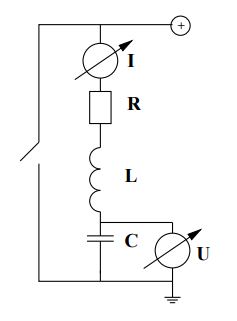
\includegraphics[scale=0.8]{Bilder/RLCSchaltung.png}
\end{center}
\caption[RLC Schaltung]{Schaltplan des RLC-Schwingkreises. (Quelle: Praktikumsskript Seite 84)}
\label{fig:RLCSchaltung}
\end{figure}

\begin{table}
\begin{center}
\begin{tabular}{|c|c|}
\hline
Messparameter &  $10 \mu s$ Messintervall;  2000 Messwerte \\
\hline
Einstellungen & Messbereich U: -10V bis 10V\\
\hline
Trigger & fallend, 6V\\
\hline
\end{tabular}
\caption[CASSY]{Einstellungen CASSY}
\label{tab:CASSY}
\end{center}
\end{table}


\subsubsection{Durchführung}
Es wird die durch Entladen des Kondensators angeregte Schwingung aufgezeichnet. Dazu wird der Kondensator zunächst mit 7V Ladespannung geladen. Nach Einstellen des Widerstandes am Potentiometer (Eingesteller Wert wurde mit dem Multimeter bestimmt) wird der Schalter geschlossen. Durch den Kurzschluss der Spannungsquelle entlädt sich der Kondensator über den Widerstand. Der Verlauf der Kondensatorspannung und des Stroms werden aufgezeichnet.\\
Der Entladevorgang wurde für jede Widerstandseinstellung insgesamt fünf mal durchgeführt.

\subsection{Auswertung Oszilloskop}
Mittels Oszilloskop wurde eine Vorauswertung bei einem gesteckten $10\Omega$ Widerstand vorgenommen. Der Kondensator wurde mit 7V geladen und der durch kurzschließen der Spannungsquelle eingeleitete Entladevorgang und die dadurch angeregte Schwingung mit dem Oszilloskop aufgezeichnet.\\
Im Oszilloskop war kein Offset der Spannung erkennbar. Für die Bestimmung wurden Minima der Spannung abgezählt. Dabei ergab sich für drei vollständige Perioden die Start- und Endwerte:
\begin{equation}
t_1=0.76ms \quad \quad t_2=8.64ms \quad \rightarrow \quad \Delta t=7.88ms
\end{equation}

Für den Fehler auf die Zeitbestimmung wurde der Cursor nach links und rechts bewegt und der erste gegenüber $t_i$ veränderte Wert notiert. Für das so entstehende Intervall wurde eine Gleichverteilung angenommen:
\begin{equation}
\sigma_{t_2}=\frac{8.64-8.52}{\sqrt{12}}ms=0.03ms \quad \quad 
\sigma_{t_1}=\frac{0.79-0.73}{\sqrt{12}}ms=0.02ms
\end{equation}

Es wurden drei Perioden erfasst. Damit ergibt sich mit $T=(t_2-t_1)/3$:

\begin{equation}
\Rightarrow \quad T=2.63ms \quad \quad \sigma_T=0.01ms
\end{equation}

Und schlussendlich für die Kreisfrequenz:
\begin{equation}
\omega=\frac{2\pi}{T}=2389Hz \quad \quad \sigma_{\omega}=\omega \frac{\sigma_T}{T}=21Hz
\end{equation}

Für die Bestimmung der Dämpfung wurden die Amplituden von vier aufeinanderfolgenden Minima abgelesen. Der Fehler ergibt sich wieder durch Bewegen des Cursors (vgl. Zeitmessung).\\
Für zwei aufeinanderfolgende Amplituden $A_n$ und $A_{n+1}$ im Abstand einer Periode gilt:
\begin{equation}
\delta_n=\frac{\ln{\frac{A_n}{A_{n+a}}}}{T}
\end{equation}

Mittels Fehlerfortpflanzung folgt:
\begin{equation}
\sigma_{\delta_n}=\delta_n \sqrt{(\frac{\sigma_{x_n}}{x_n \ln{x_n}})^2+(\frac{\sigma_T}{T})^2} \quad \text{mit} \quad x_n=\frac{A_n}{A_{n+a}} \rightarrow \sigma_{x_n}=x_n\cdot \sqrt{(\frac{\sigma_{A_n}}{A_n})^2+(\frac{\sigma_{A_{n+1}}}{A_{n+1}})^2}
\end{equation}

Eine Zusammenfassung von Amplituden und Werten für die Dämpfung findet sich in Tab.\ref{tab:DämpfungOszi}
\begin{table}
\begin{center}
\begin{tabular}{|c|c|c|c|}
\hline
n & $U_n[V]$ & $\delta_n[1/ms]$ & $\sigma_{\delta_n}[ms]$\\
\hline
1 & $-4.96 \pm 0.03$ & 0.28 & 0.01\\
\hline
2 & $-2.40 \pm 0.05$ & 0.29 & 0.02\\
\hline
3 & $-1.12 \pm 0.03$ & 0.26 & 0.03\\
\hline
4 & $-0.56 \pm 0.03$ & - & -\\
\hline
\end{tabular}
\end{center}
\caption{Dämpfungswerte bei der Auswertung mittels Oszilloskop}
\label{tab:DämpfungOszi}
\end{table}

Die Ergebnisse der Dämpfung werden in einem gewichteten Mittelwert zusammengefasst zu $\delta=(0.28 \pm 0.01)kHz$.



\subsection{Auswertung CASSY}
\subsubsection{Rohdaten}
Der prinzipielle Verlauf ist bei fast allen Messungen weitesgehend identisch (gedämpfte Schwingung/Exponentieller Abfall), deswegen werden hier nur einige Spannungsverläufe exemplarisch gezeigt (Abb. \ref{fig:Spannung19,6})


\begin{figure}
\begin{center}
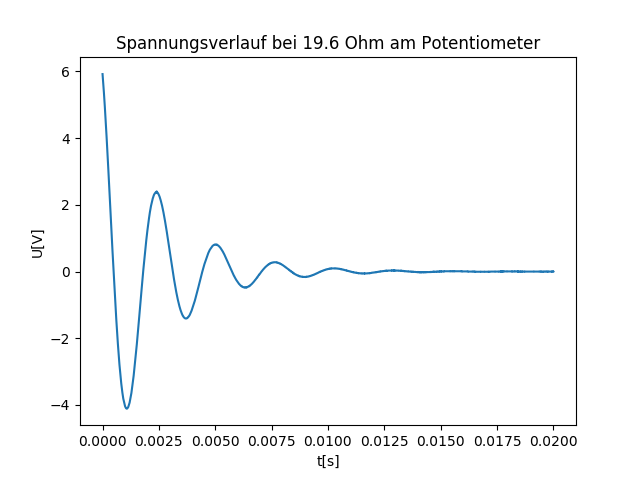
\includegraphics[scale=0.5]{Bilder/Spannungsverlauf19,6Ohm}
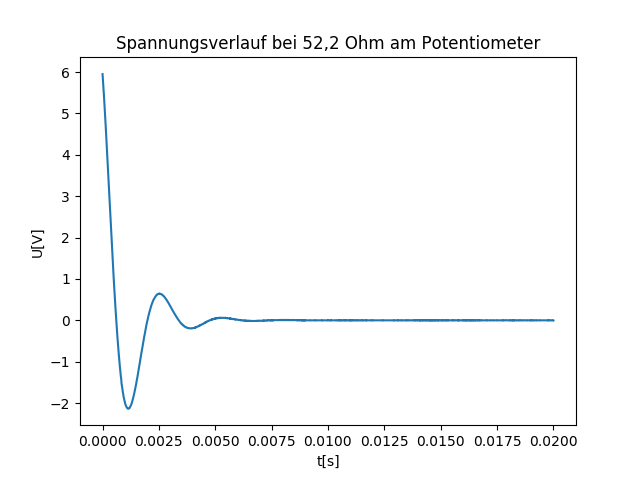
\includegraphics[scale=0.5]{Bilder/Spannungsverlauf52,2Ohm}
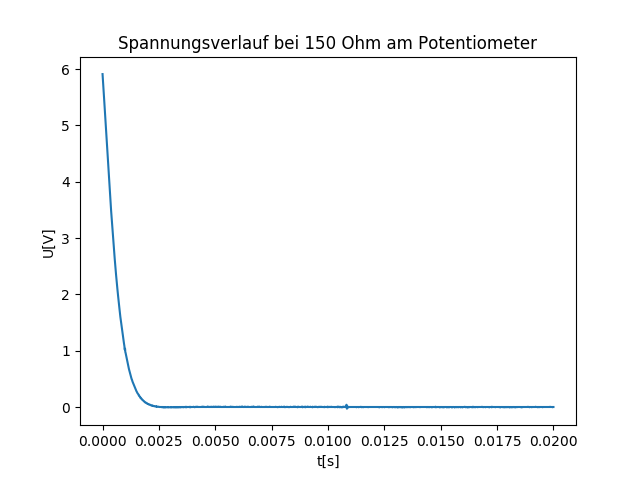
\includegraphics[scale=0.5]{Bilder/Spannungsverlauf150Ohm}
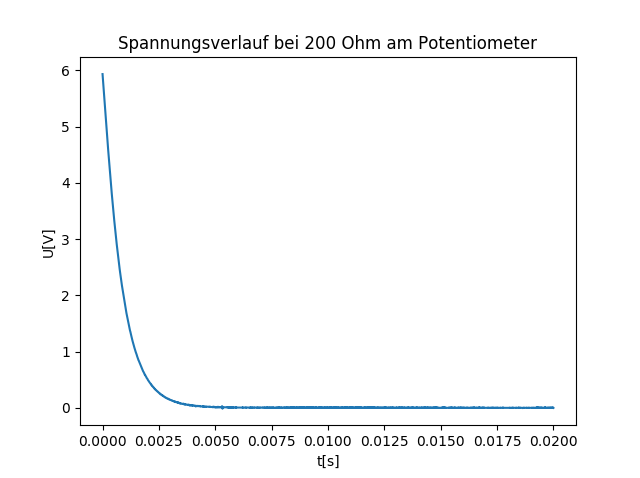
\includegraphics[scale=0.5]{Bilder/Spannungsverlauf200}
\end{center}
\caption[Spannungsverlauf]{Spannungssignal für verschiedene Einstellungen des Potentiometers (Wert vom Multimeter).}
\label{fig:Spannung19,6}
\end{figure}



\subsubsection{Frequenzbestimmung}
In diesem Versuch stehen einem prinzipiell zwei Möglichkeiten zur Frequenzbestimmung zur Verfügung.
Einmal durch Fouriertransformation des gemessenen Spannungssignals und anschließender Peakbestimmung, die zweite Möglichkeit durch Bestimmung der mittleren Periodendauer des Spannungssignals.\\

Die Bestimmung mittels Fouriertransformation ist in diesem Fall nicht zufriedenstellend, da die Auflösung des Spektrums zu grob ist (siehe Abb.\ref{fig:Fourier19,6} für das zu Abb.\ref{fig:Spannung19,6} zugehörige Frequenzspektrum).\\

\begin{figure}
\begin{center}
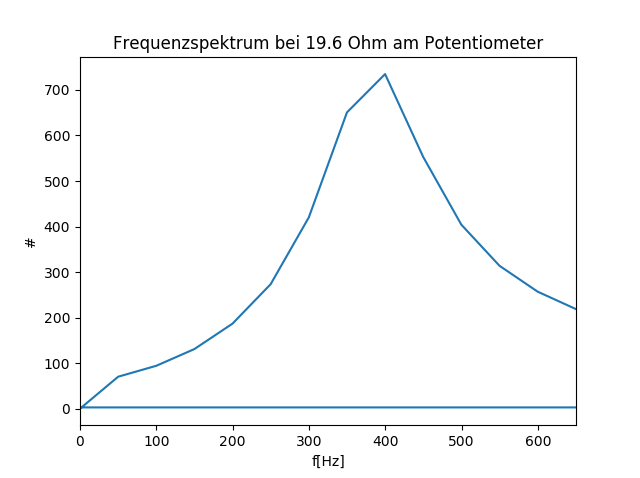
\includegraphics[scale=0.75]{Bilder/fft_19,6Ohm}
\end{center}
\caption{Frequenzspektrum von Messung 1 bei $R=19.6 \Omega$. Die Auflösung ist mit $\approx 50Hz$ viel zu grob.}
\label{fig:Fourier19,6}
\end{figure}

Für die Bestimmung der Frequenz aus der mittleren Periodendauer sind bessere Ergebnisse erzielt worden.\\
Dazu wurden im Spannungssignal Vorzeichenwechsel gesucht. Die Nullstelle ist dann der Mittelwert der Zeitpunkte eines solchen Vorzeichenwechsels, als Fehler auf die Nullstelle wurde eine Gleichverteilung zwischen den beiden Zeitpunkten angenommen. Es ergibt sich dann für Nullstellen $t_i$:

\begin{equation}
t_i=(t_++t_-)/2 \quad \quad \quad
\sigma_{t_i}=\frac{t_+-t_-}{\sqrt{12}}
\end{equation}

Mit der Zeitspanne zwischen zwei Nullstellen ergibt sich für die Periodendauer:

\begin{equation}
T_i=2\cdot (t_{i+1}-t_i) \quad \quad
\sigma_{T_i}=2\cdot \sqrt{\sigma_{t_{i+1}}^2+\sigma_{t_i}^2}
\end{equation}

Mittels Mittelwert und Fehler auf diesen ergibt sich für jede der fünf Messungen pro eingestelltem Widerstand eine mittlere Periodendauer mit Fehler. Mittels einem gewichteten Mittelwert werden diese zu einem Endergebnis für jede Widerstandseinstellung zusammengefasst.\\
Für die Frequenz folgt dann:

\begin{equation}
f=\frac{1}{\overline{T}} \quad \quad \quad
\sigma_f=\frac{\sigma_{\overline{T}}}{\overline{T}^2}
\end{equation}

Eine Zusammenstellung der auf diese Weise gewonnen Frequenzen bei diversen Widerstandseinstellungen finden sich in Tabelle \ref{tab:Frequenzen}. Für größere Widerstände ist eine Frequenzbestimmung auf diese Weise nicht mehr gelungen.

\begin{table}
\begin{center}
\begin{tabular}{|c|c|c|}
\hline
$R[\Omega]$ & $f[Hz]$ & $\sigma_f[Hz]$ \\
\hline
 19.6 & 382.78 & 0.16\\
\hline
 28.5 & 376.84 & 0.18\\
\hline
 38.9 & 373.21 & 0.20\\
\hline
 52.2 & 364.84 & 0.22\\
\hline
 68.8 & 350.75 & 0.24\\
\hline
\end{tabular}
\end{center}
\caption{Ergebnisse der Frequenzbestimmung durch Nullstellen}
\label{tab:Frequenzen}
\end{table}



\subsubsection{Bestimmung der Dämpfungskonstanten}
Die Dämpfungskonstante $\delta$ kann auf zwei verschiedene Weisen bestimmt werden.\\

Erstes Verfahren:\\
Da die Amplitude der Kondensatorspannung $U_C(t)$ mit der Zeit exponentiell abfällt, gilt für das Verhältnis der Amplituden $A_n$:
\begin{equation}
A_{n+1} = A_n \cdot e^{-\delta \cdot (t_{n+1} - t_n)} \quad \rightarrow \quad \delta_n = \frac{\ln ( A_n / A_{n+1})}{t_{n+1}-t_n}
\end{equation}

So erhält man aus jeder Messung eine mittlere Dämpfungskonstante. Diese kann man noch über die 5 Messungen mitteln, die wir je Widerstand durchführten. Der statistische Fehler auf $\delta$ ergibt sich aus der linearen Regression, der systematische Fehler ist Null.\\

Zweites Verfahren:\\
Man erhält die Dämpfungskonstante $\delta$ und deren Fehler $\sigma_\delta$ aus der Anpassung einer Einhüllenden an die Messung der Kondensatorspannung $U_C(t)$. So ergibt sich der statistische Fehler ebenfalls aus der Anpassung und den systematischen Fehler erhält man durch die Verschiebemethode.  Die Ergebnisse finden sich in Tabelle \ref{tab:delta}.

\begin{table}
	\centering
	\begin{tabular}{|c|c|c|c|}
		\hline
		\textbf{Widerstand [$\Omega$]} & \textbf{$\delta_1 \pm \sigma_{stat} [1/s]$} & \textbf{$\delta_2 \pm \sigma_{stat} \pm \sigma_{sys} [1/s]$} & \textbf{Mittelwert [1/s]} \\
		\hline
		19.6 & 370.3 $\pm$ 5.3 & 397.9 $\pm$ 0.1 $\pm$ 14.4 & 373.5 $\pm$ 5.0 \\
		\hline
		28.5 & 506.4 $\pm$ 9.9 & 526.4 $\pm$ 0.2 $\pm$ 23.9 & 509.3 $\pm$ 9.1 \\
		\hline
		38.9 & 694.8 $\pm$ 16.4 & 671.9 $\pm$ 0.4 $\pm$ 35.3 & 690.8 $\pm$ 14.9 \\
		\hline
		52.2 & 820.1 $\pm$ 26.4 & 820.2 $\pm$ 0.8 $\pm$ 51.5 & 820.2 $\pm$ 23.5 \\
		\hline
		68.6 & 1010.5 $\pm$ 25.9 & 1087.1 $\pm$ 0.7 $\pm$ 79.4 & 1017.9 $\pm$ 24.6 \\
		\hline
	\end{tabular}
	\caption{Ergebnisse für die Dämpfungskonstanten nach gestecktem Widerstand}
	\label{tab:delta}
\end{table}


\subsubsection{Berechnung von R, L und C}
Aus der Differentialgleichung des RLC-Schwingkreises folgt:
\begin{equation}
\delta = \frac{R_{gesamt}}{2L} \quad \rightarrow \quad R_{gesteckt} = 2 L \cdot \delta - (R_L + R_{Rest})
\end{equation}
Trägt man also den gesteckten Widerstand $R_{gesteckt}$ gegen die Dämpfungskonstante $\delta$ auf, erhält man als Steigung der angepassten Geraden $m = 2L$ und als y-Achsenabschnitt $b = R_{Rest}$. Unsere Messungen ergaben L = (35.8$\pm$2.1)mH und $R_L + R_{Rest}$ = (7.4 $\pm$ 2.0)$\Omega$ (Abbildung \ref{pic:fit_L_RLC}).

\begin{table}[H]
	\centering
	\begin{tabular}{|c|c|c|c|}
		\hline
		- & \textbf{Gemessen} & \textbf{Brücke} & \textbf{Herstellerangabe} \\
		\hline
		Induktivität [mH] & 35.8 $\pm$ 2.1 & 36.2 & 35 \\
		\hline
	\end{tabular}
\end{table}

\begin{figure}
	\centering
	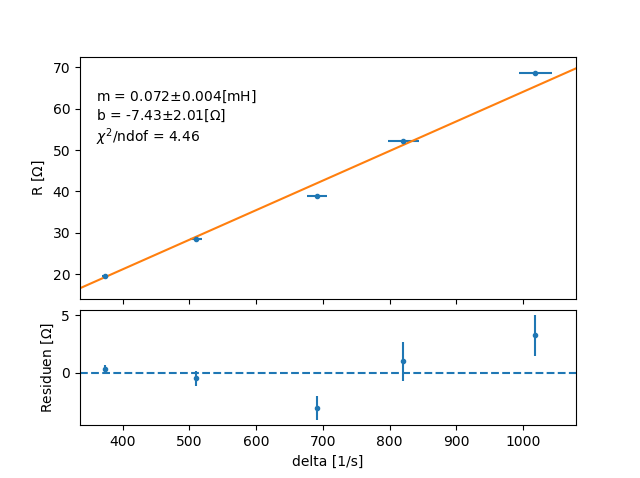
\includegraphics[width=0.8\linewidth]{Bilder/fit_L_RLC}
	\caption{Gesteckter Widerstand gegen Dämpfungskonstante}
	\label{pic:fit_L_RLC}
\end{figure}

Weiterhin kann man dann die Kapazität bestimmen, indem man das Quadrat der Kreisfrequenz $\omega$ gegen das Quadrat der Dämpfungskonstante $\delta$ aufträgt.
\begin{equation}
\omega^2 = \omega_0^2 -\delta^2 = \frac{1}{LC} - \delta^2
\end{equation}
Passt man eine Gerade mit Steigung -1 an diese Daten an, erhält man als y-Achsenabschnitt $y = \frac{1}{LC}$.

Für unsere Daten ergab dies C = (4.72$\pm$0.28)$\mu F$ (siehe Abbildung \ref{pic:fit_C_RLC}).

Sowohl für die Spule, als auch den Kondensator stimmen die von uns bestimmten Werte, die Angaben des Hersteller und gegebenenfalls der an der Brücke gemessene Wert sehr gut überein.


\begin{table}[H]
	\centering
	\begin{tabular}{|c|c|c|c|}
		\hline
		- & \textbf{Gemessen} & \textbf{Herstellerangabe} \\
		\hline
		Kapazität [$\mu F$] & 4.72 $\pm$ 0.28 & 4.7 \\
		\hline
	\end{tabular}
\end{table}

\begin{figure}
	\centering
	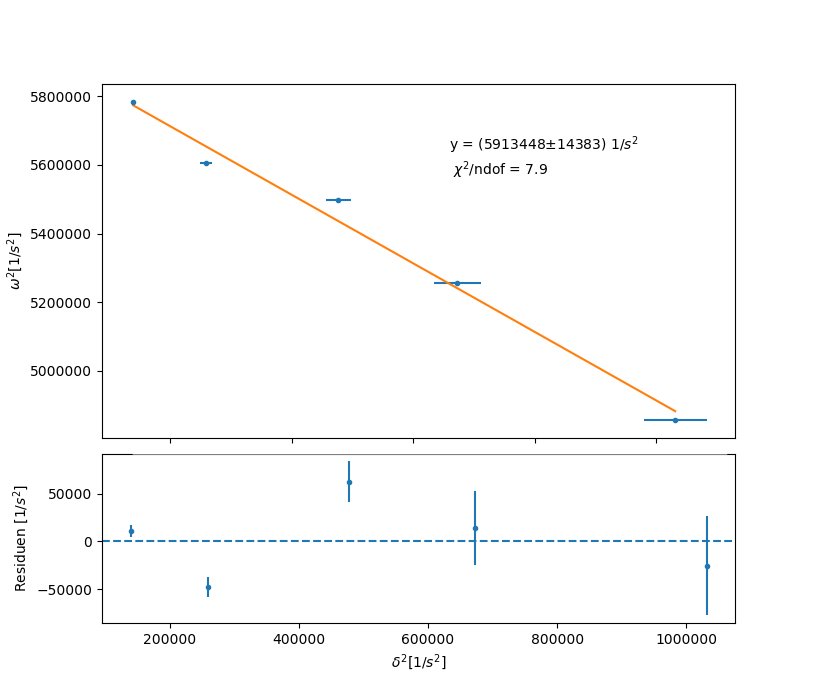
\includegraphics[width=0.8\linewidth]{Bilder/fit_C_RLC}
	\caption{$\omega^2$ gegen $\delta^2$ mit angepasster Geraden der Steigung -1.}
	\label{pic:fit_C_RLC}
\end{figure}


\subsubsection{Aperiodischer Grenzfall}
Bei einer nominellen Einstellung von $R_{gesteckt}=0.150k\Omega$ am Potentiometer kam der zeitliche Verlauf des Spannungssignals dem aperiodischen Grenzfall am nächsten. Aus zeitlichen Gründen war es nicht möglich den Bereich mit einer feineren Einstellung abzutasten um sich dem Grenzfall noch besser zu nähern.\\
Es wurde versucht zwei Einhüllende anzupassen, so dass der gemessene Verlauf möglichst innerhalb der Einhüllenden verbleibt. Die beste Einhüllung ergab sich für $R=185\Omega$ und $R=200\Omega$, wobei $L=35.8mH$ verwendet wurden. (vgl. Abb.\ref{fig:Aperiodisch} )

\begin{figure}
\begin{center}
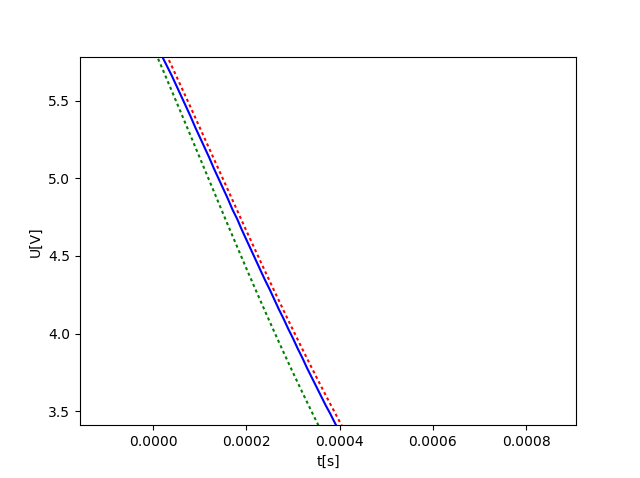
\includegraphics[scale=0.4]{Bilder/Aperiodisch1}
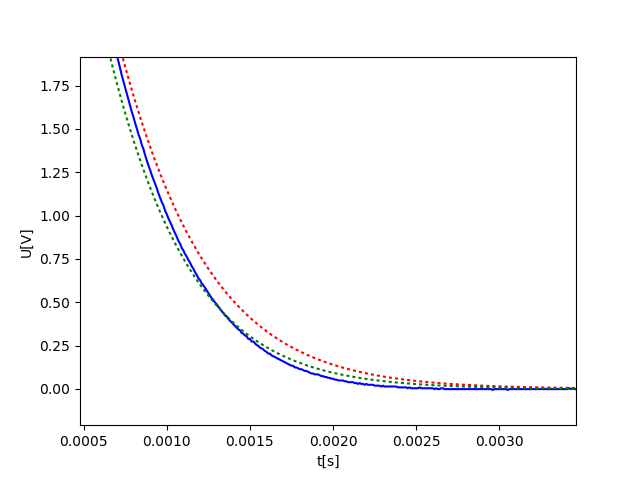
\includegraphics[scale=0.4]{Bilder/Aperiodisch2}
\end{center}
\caption{Zoom auf zwei Bereiche. Das gemessene Spannungssignal ist durchgezogen gezeichnet. Im zweiten Bild ist der einzige Bereich gezeigt indem das Einhüllen wenig gut gelingt.}
\label{fig:Aperiodisch}
\end{figure}

Als Widerstand des aperiodischen Grenzfalls wird der Mittelwert der beiden Einhüllungswiderstände verwendet, als Fehler wird ein Gleichverteilungsfehler zwischen den Widerständen angenommen. Damit erhält man:
\begin{equation}
R_{ap}=192.5\Omega \quad \quad \sigma_{R_{ap}}=4.3\Omega
\end{equation}

Den Wert den man erwarten würde ergibt sich aus der Kapazität und der Induktivität:
\begin{equation}
R_{ap}=2\cdot \sqrt{\frac{L}{C}}=2\sqrt{\frac{35.8mH}{4.7\mu F}}=174.6\Omega
\end{equation}

Und für den Fehler:

\begin{equation}
\sigma_{R_{ap}}=\sqrt{\frac{\sigma_L^2}{CL}+\frac{\sigma_C^2 L}{C^3}}=5.1 \Omega
\end{equation}

Die relativ große Abweichung von etwa 4.2 Standardabweichungen zum erwarten Wert ist wahrscheinlich darauf zurückzuführen, dass es sich bei dem Spannungsverlauf an dem die Anpassung von Einhüllenden vorgenommen wurde nur um die beste Approximation des aperiodischen Grenzfalls handelt. Bei besserer Abtastung und besserer Annäherung an den Grenzfall wäre dann zu erwarten, dass der dann bestimmte Widerstandswert näher an der Erwartung liegt.

\subsection{Fazit}
Durch die Bestimmung von Schwingungsfrequenzen und Dämpfung aus den aufgezeichneten Schwingungen konnten wir die Induktivität der Spule sowie die Kapazität des Kondensators mit einer Genauigkeit von etwa 6\% messen.\\
Der Restwiderstand der Schaltung konnte hingegen nur auf 27\% genau bestimmt werden.\\
Herstellerangaben und von uns bestimmte Werte weichen dabei in der Regel um weniger als eine Standardabweichung voneinander ab.\\
Lediglich die Aufzeichnung und Bestimmung des aperiodischen Grenzfalls ist nicht vollständig gelungen. Der bestimmte Wert weicht um mehrere Standardabweichungen von der theoretischen Vorhersage ab. Ursächlich dafür ist wahrscheinlich, dass eine exakte Aufzeichnung des Grenzfalls nicht gelungen ist und mit der besten vorhandenen Approximation gearbeitet werden musste.


\newpage
\section{Gekoppelte Schwingkreise - Schwebung}
\subsection{Versuchsbeschreibung}
Ein LC-Schwingkreis kann induktiv mit einem zweiten LC-Schwingkreis gekoppelt werden, der dadurch zu erzwungenen Schwingungen angeregt wird. Falls die Eigenfrequenzen der Schwingkreise gleich ist $w_1 = w_2$, tritt eine Resonanz auf. In diesem Fall kann eine Schwebung beobachtet werden. Bedeutet: Die Schwingungsenergie "schwingt" zwischen den Schwingkreisen hin und her. \\
Bei diesem Versuch werden die Fundamentalschwingungen und die Schwebung zweier gekoppelter Schwingkreise aufgenommen. Die Differentialgleichungen der gekoppelten Schwingkreise lauten:
\begin{equation}
\ddot{I_1} + k \cdot \ddot{I_2} + \dfrac{I_1}{L \cdot C} = 0
\end{equation}
\begin{equation}
\ddot{I_2} + k \cdot \ddot{I_1} + \dfrac{I_2}{L \cdot C} = 0
\end{equation}
mit Kopplung k ($0 < k < 1)$ folgen die Eigenfrequenzen zu
\begin{equation}
\dfrac{w_0}{\sqrt{1+k}} = w_+ < w_0 < w_- = \dfrac{w_0}{\sqrt{1-k}} 
\end{equation}
Dabei ist $w_0$ die Eigenfrequenz des Schwingkreises im ungekoppelten Fall ($w_0 = \dfrac{1}{\sqrt{LC}}$)
Die Kopplung kann aus den Frequenzen der Fundamentalschwingungen berechnet werden:
\begin{equation}
k = \dfrac{f_-^2 - f_+^2}{f_-^2 + f_+^2}
\label{eq:Kopplung}
\end{equation}
\\ Die Erwartung bei dieser Versuchskonfiguration ist, dass die Amplitudennullstellen des einen Schwingkreises mit einem Amplitudenextremum des anderen zusammenfallen. Die Dämpfung durch Ohm'sche Widerstände in allen Bauteilen verschiebt diese beiden allerdings gegeneinander. Für Kopplungen k < 0,2 lässt sich die Verschiebung näherungsweise berechnen:
\begin{equation}
\Delta t \approx \dfrac{1}{w_{Schwebung}} \cdot \left[\dfrac{\pi}{2} - \arctan \left( \dfrac{k}{R} \cdot \sqrt{\dfrac{L}{C}} \right)\right]
\label{eq:delta_t}
\end{equation}
\subsection{Aufbau und Durchführung}
\begin{figure}
\begin{center}
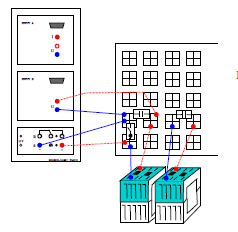
\includegraphics[scale=1.2]{Bilder/Schwebung_Aufbau.PNG}
\end{center}
\caption[Aufbau Schwebung]{Aufbau für Messung der Schwebung zweier gekoppelter Schwingkreise}
\label{fig:Schwebung_Aufbau}
\end{figure}
Abbildung \ref{fig:Schwebung_Aufbau} zeigt den Aufbau. Es werden zwei LC-Schwingkreise von einander getrennt aufgebaut. Dabei wird nur eine Spannungsquelle verwendet, die einen der beiden Kondensatoren auflädt. Anschließend werden die beiden Spulen direkt nebeneinander gestellt, wie im Bild zu sehen. \\
Mit der Spannungsquelle wird einer der beiden Kondensatoren aufgeladen (der andere bleibt ungeladen). Anschließend wird mittels eines Schalters die Spannungsquelle kurzgeschlossen. Mithilfe eines Triggers wird die Messung gleichzeitig gestartet. \\
Die CASSY Einstellungen sind: \\
\begin{center}
\begin{tabular}{|c|c|}
\hline 
Messintervall & 10 $\mu s$ \\ 
\hline 
Messwerte & 16000 \\ 
\hline 
Messbereich Spannung & $|U| \leq 3V$ \\ 
\hline 
\end{tabular}
\end{center}

Die verwendeten Spulen wurden mit der Brücke vermessen: \\
\begin{center}
\begin{tabular}{|c|c|c|}
\hline 
Spule 1 & (9,047 $\pm$ 0,023 $\pm$ 0,001) mH & (2,85 $\pm$ 0,01 $\pm$ 0,01) $\Omega$ \\ 
\hline 
Spule 2 & (9,123 $\pm$ 0,023 $\pm$ 0,001) mH & (2,77 $\pm$ 0,01 $\pm$ 0,01) $\Omega$ \\ 
\hline 
\end{tabular} 
\end{center}

\subsection{Auswertung}
\subsubsection{Rohdaten}
\begin{figure}
\begin{center}
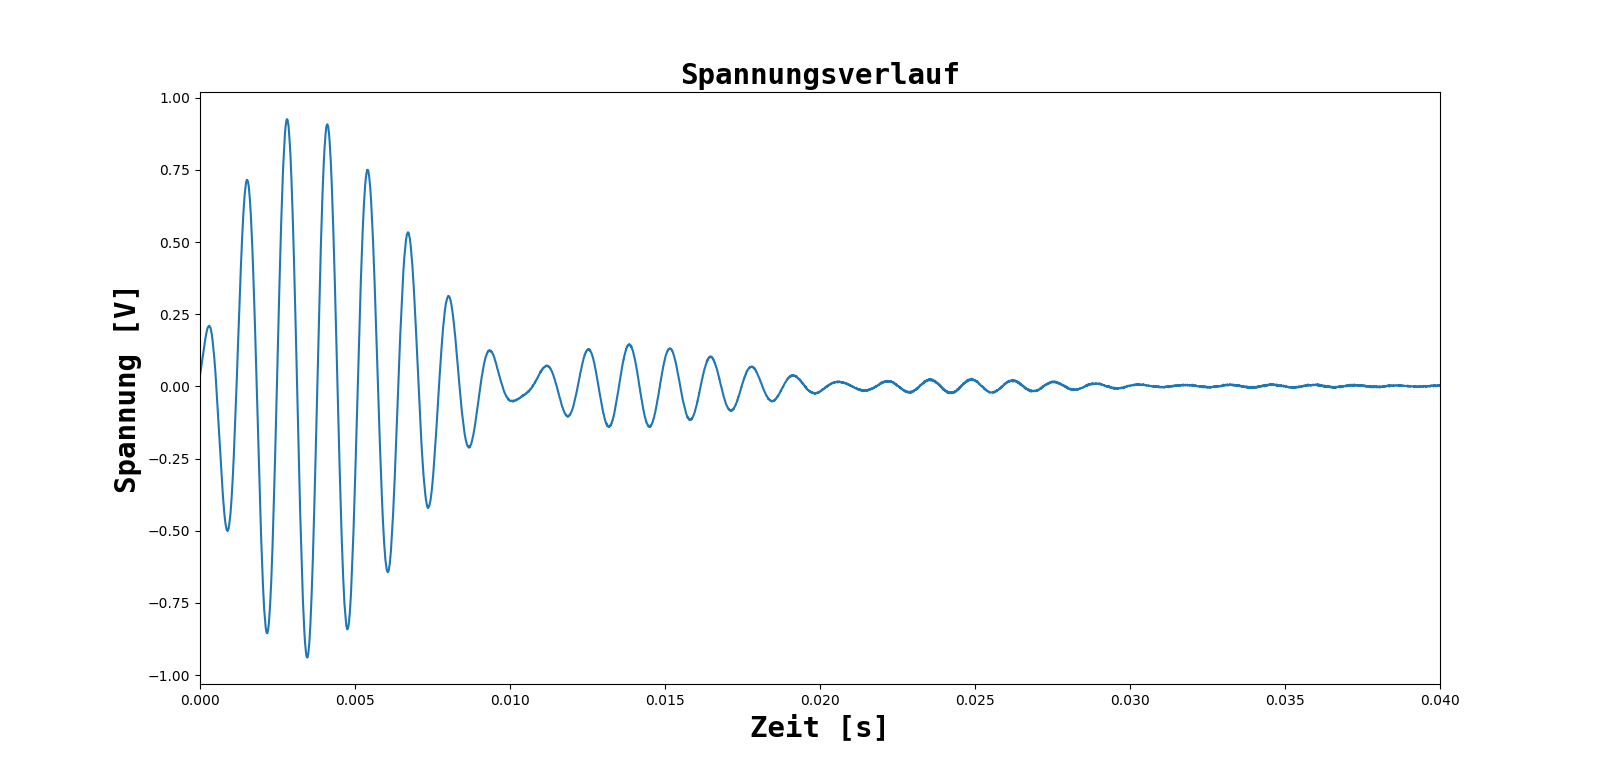
\includegraphics[scale=0.4]{Bilder/Schwebung_Rohdaten.png}
\end{center}
\caption[Rohdaten Schwebung]{Rohdaten der Messung zweier gekoppelter Schwingkreise}
\label{fig:Schwebung_Roh}
\end{figure}
Abbildung \ref{fig:Schwebung_Roh} zeigt die Rohdaten der Messung in Form von dem zeitlichen Spannungsverlauf. Die Schwebung ist hier bereits gut zu sehen.  

\subsubsection{Fouriertransformation}
\begin{figure}
\begin{center}
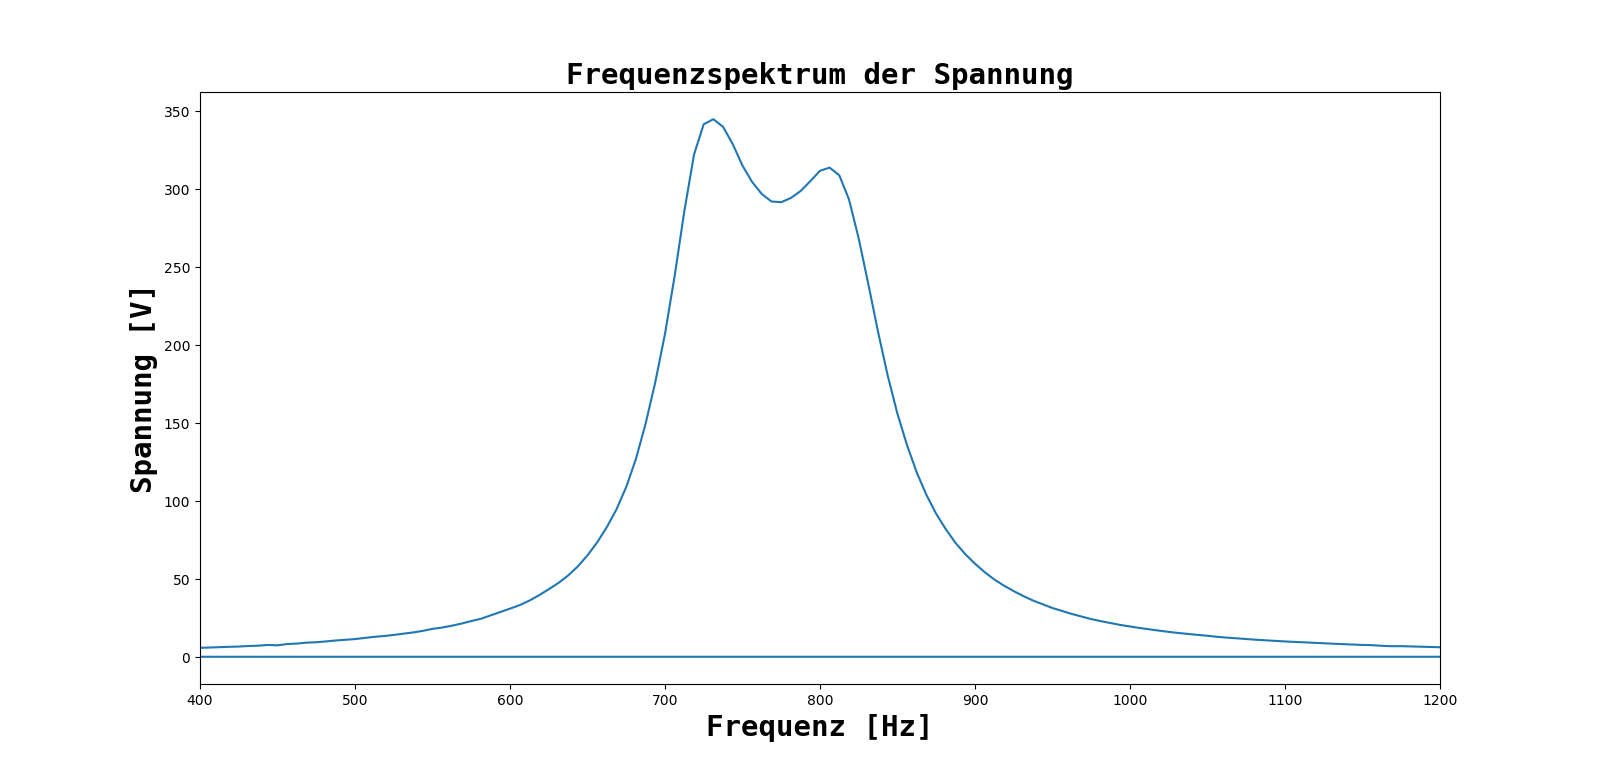
\includegraphics[scale=0.4]{Bilder/Schwebung_Frequenzspektrum.png}
\end{center}
\caption[Frequenzspektrum Schwebung]{Frequenzspektrum der Schwingung zweier gekoppelter Schwingkreise}
\label{fig:Schwebung_Frequenzspektrum}
\end{figure}
Um die Frequenzen der Schwingung zu erhalten, wird auf die Rohdaten eine Fouriertransformation angewandt. Hier wurde die Fast-Fourier-Transformation (kurz: FFT) verwendet. Diese ist deutlich schneller als die eigentliche Fouriertransformation und liefert in diesem Fall auch dieselben Ergebnisse (das wurde stichprobenartig überprüft). Abbildung \ref{fig:Schwebung_Frequenzspektrum} zeigt das Frequenzspektrum der Schwingung. Die beiden Peaks sind zwar gut zu sehen, allerdings auch nicht sehr gut voneinander getrennt bzw. die Amplitude sinkt zwischen den beiden Peaks nur wenig ab.

\subsubsection{Ergebnis und Fazit}
Der beschriebene Versuch wurde mit 3 verschiedenen Kopplungen durchgeführt: Einmal wurden die Spulen direkt nebeneinander gestellt (1), einmal mit etwa einer handbreit Abstand (2) und einmal direkt nebeneinander mit einem gemeinsamen Eisenkern(3). \\
Die Kopplung wurde jeweils mit Gleichung \ref{eq:Kopplung} bestimmt. Der Fehler ergibt sich aus der gauß'schen Fehlerfortpflanzung zu:
\begin{equation}
\sigma_k = \sqrt{\left( \left( \dfrac{2 \cdot f_-}{f_+^2 + f_-^2} - 2 \cdot f_- \cdot \dfrac{f_-^2 - f_+^2}{(f_+^2 + f_-^2)^2} \right) \cdot \sigma_{f_-} \right)^2 + \left( \left( \dfrac{2 \cdot f_+}{f_+^2 + f_-^2} + 2 \cdot f_+ \cdot \dfrac{f_-^2 - f_+^2}{(f_+^2 + f_-^2)^2} \right) \cdot \sigma_{f_+} \right)^2}
\label{eq:Kopplung_k}
\end{equation}
Außerdem wurde die Zeitverschiebung aus den Daten jeweils über den zeitlichen Abstand zwischen einem Extremum in der einen und einer Nullstelle in der anderen Spannung bestimmt. Berechnet man die Zeitverschiebung mit Gleichung \ref{eq:delta_t}, so findet man mit der gauß'schen Fehlerfortpflanzung den Fehler auf $\Delta t$ zu:
\begin{equation}
\sigma_{\Delta t} = \sqrt{\left( \dfrac{d(\Delta t)}{dk} \cdot \sigma_k \right)^2 + \left( \dfrac{d(\Delta t)}{dR} \cdot \sigma_R \right)^2 + \left( \dfrac{d(\Delta t)}{dL} \cdot \sigma_L \right)^2 + \left( \dfrac{d(\Delta t)}{dR} \cdot \sigma_R \right)^2}
\end{equation}
mit
\[\dfrac{d(\Delta t)}{dk} = \dfrac{-1}{2 \cdot \pi \cdot f_s} \cdot \dfrac{1}{R} \cdot \sqrt{\dfrac{L}{C}} \cdot \dfrac{1}{1 + \left( \dfrac{k}{R} \right)^2 \cdot \dfrac{L}{C}} \]
\[\dfrac{d(\Delta t)}{dR} = \dfrac{1}{2 \cdot \pi \cdot f_s} \cdot \dfrac{k}{R^2} \cdot \sqrt{\dfrac{L}{C}} \cdot \dfrac{1}{1 + \left( \dfrac{k}{R} \right)^2 \cdot \dfrac{L}{C}} \]
\[\dfrac{d(\Delta t)}{dC} = \dfrac{1}{4 \cdot \pi \cdot f_s} \cdot \dfrac{k}{R} \cdot \sqrt{\dfrac{L}{C^3}} \cdot \dfrac{1}{1 + \left( \dfrac{k}{R} \right)^2 \cdot \dfrac{L}{C}} \]
\[\dfrac{d(\Delta t)}{dL} = \dfrac{-1}{4 \cdot \pi \cdot f_s} \cdot \dfrac{k}{R} \cdot \sqrt{\dfrac{1}{L \cdot C}} \cdot \dfrac{1}{1 + \left( \dfrac{k}{R} \right)^2 \cdot \dfrac{L}{C}} \]

Die Ergebnisse für k und $\Delta t$ sowie der errechnete Erwartungswert für $\Delta t$ finden sich in nachfolgender Tabelle: \\

\begin{center}
\begin{tabular}{|c|c|c|c|c|}
\hline 
Messung & $k_{gemessen}$ & $\Delta t_{berechnet}$ [ms] & $\Delta t_{gemessen}$ [s] & $\Delta t_{berechnet} - \Delta t_{gemessen}$  \\ 
\hline 
(1) & 0,13029 $\pm$ 0,00069 & 1,49 $\pm$ 0,35 & 0,33 $\pm$ 0,44 & 2,6 $\sigma$ \\ 
\hline 
(2) & 0,08780 $\pm$ 0,00081 & 3,06 $\pm$ 0,63 & 0,31 $\pm$ 0,32 & 8,6 $\sigma$ \\ 
\hline 
(3) & 0,20731 $\pm$ 0,00003 & 0,62 $\pm$ 0,16 & 0,76 $\pm$ 1,62 & 0,1 $\sigma$ \\ 
\hline 
\end{tabular} 
\end{center}

Die Kopplung der beiden Schwingkreise konnte durch die Bestimmung der beiden Frequenzen aus dem Frequenzspektrum der Schwingung der Spannung sehr gut bestimmt werden (insbesondere mit kleinem Fehler). Einen Vergleichswert anzugeben gestaltet sich an dieser Stelle als recht schwierig, da dafür viele Faktoren eine Rolle spielen. \\
Die Bestimmung der Zeitverschiebung zwischen den beiden Schwingungen durch Bestimmung der zeitlichen Differenz zwischen einem Extremum in der einen und einer Nullstelle in der anderen Spannung hat nicht so gut funktioniert. Liegen die Werte zum Teil zwar nur wenige Standardabweichungen von den errechneten Werten entfernt, so liegt dies doch daran, dass die Fehler recht groß sind.
\newpage
\section{Gekoppelte Schwingkreise Teil 2 - Fundamentalschwingungen}
\subsection{Versuchsbeschreibung}
In diesem Teilversuch sollen nun die Fundamentalschwingungen bestimmt werden. Dazu werden zwei über die Spulen gekoppelte baugleiche Schwingkreise einmal gleichläufig und einmal gegenläufig angeregt.

Bei gleicher Anregung werden die Ströme addiert, was dazu führt, dass die resultierende Fundamentalschwingung gegeben ist durch
\begin{equation}
\omega_+ =\dfrac{\omega_0}{\sqrt{1+k}}
\end{equation}
wobei $\omega_0 = \dfrac{1}{\sqrt{L\cdot C}}$ die ungekoppelte Frequenz und k der Kopplungsfaktor ist.\\
Bei entgegengesetzter Anregung werden die Ströme subtrahiert. Damit ist die Frequenz:
\begin{equation}
\omega_- =\dfrac{\omega_0}{\sqrt{1-k}}
\end{equation}
\\
Der Kopplungsfaktor k kann nun wie im vorherigen versuchsteil bestimmt werden durch
\begin{equation}
k = \dfrac{f_-^2 - f_+^2}{f_-^2 + f_+^2}
\label{eq:Kopplung2}
\end{equation}

\subsection{Aufbau und Durchführung}

\begin{figure}
\begin{center}
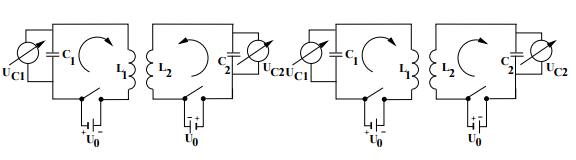
\includegraphics[width=\linewidth]{Bilder/Fund_Aufbau.PNG}
\end{center}
\caption[Aufbau Schwebung]{Aufbau für Messung der Schwebung zweier gekoppelter Schwingkreise}
\label{fig:Fund_Aufbau}
\end{figure}

Der Aufbau ist ähnlich zu dem von Teil 1, nur wird jetzt an beiden Schwingkreisen eine Spannung angelegt. Es sollte auch hier vor allem darauf geachtet werden, dass die Schwingkreise möglichst identische Bauteile haben.
Bei dem gleichsinnigen Schwingkreis sollten diese in unterschiedliche Richtung gepolt sein, im gegensinnigen in die gleiche Richtung. Da es oft schwer ist, die Windungsrichung der Spulen herauszufinden, kann während der Messung einfachheitshalber eine Spule umgepolt werden und erst bei der Auswertung analysiert werden, welcher Aufbau nun der gleichsinnige und welcher der gegensinnige war.\\
In dem von uns gewählten Aufbau standen die Spulen dicht hintereinander. Es wurde kein Eisenkern benutzt.\\
\\
Bei der Durchführung sollte möglichst bei beiden Spannungsquellen die gleichen Werte eingestellt werden. Die Schwingungen werden gleichzeitig über einen Schalter gestartet.\\
\\
Es wurden die gleichen Messeinstellungen wie bei Teil 1 verwendet.

\subsection{Auswertung}

\subsubsection{Rohdaten und Frequenzspektren}
\begin{figure}
\begin{center}
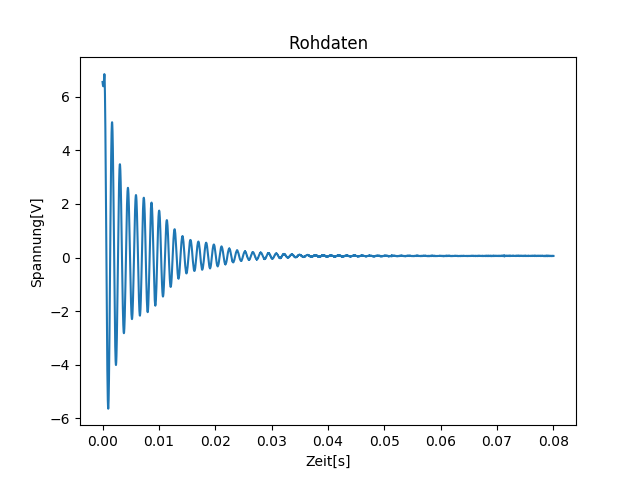
\includegraphics[width=0.49\linewidth]{Bilder/Fund_Rohdaten1.PNG}
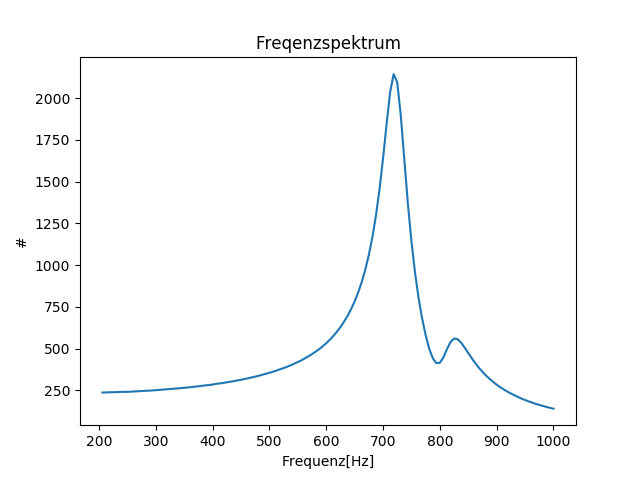
\includegraphics[width=0.49\linewidth]{Bilder/Fund_Frequenz1.PNG}
\end{center}
\caption[Aufbau Schwebung]{Rohdaten und dazugehörige FFT der Fundamentalschwingung $\omega_+$, gemessen am 1.Schwingkreis}
\label{fig:Fund_Roh1}
\end{figure}

\begin{figure}
\begin{center}
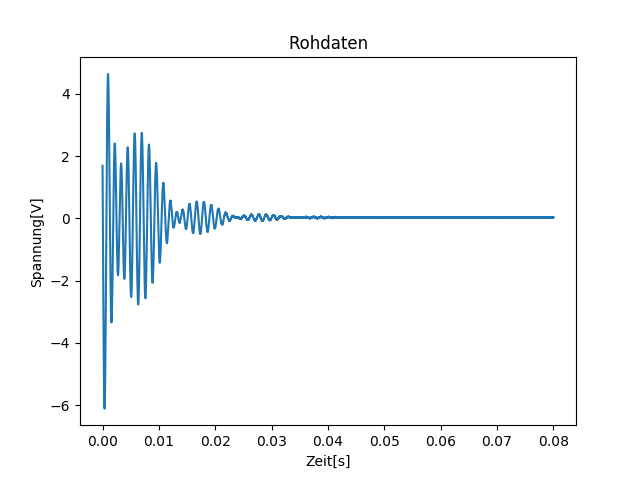
\includegraphics[width=0.49\linewidth]{Bilder/Fund_Rohdaten2.PNG}
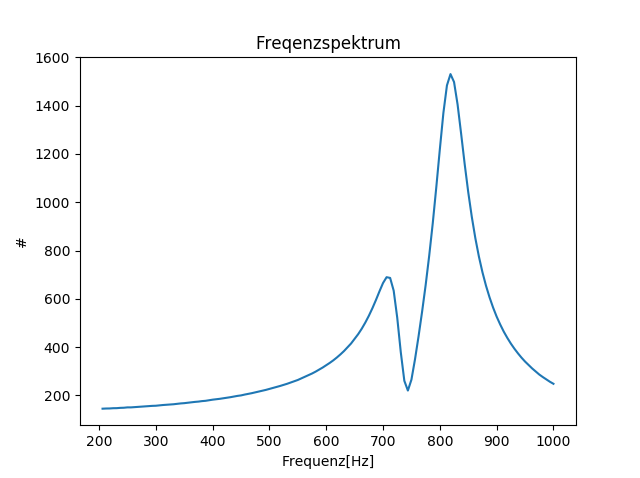
\includegraphics[width=0.49\linewidth]{Bilder/Fund_Frequenz2.PNG}
\end{center}
\caption[Aufbau Schwebung]{Rohdaten und dazugehörige FFT der Fundamentalschwingung $\omega_-$, gemessen am 1.Schwingkreis}
\label{fig:Fund_Roh2}
\end{figure}

Abb.\ref{fig:Fund_Roh1} zeigt einen ausgewählten Rohdatenplot und die dazugehörige FFT der niedrigeren Frequenz $\omega_+$. Abb.\ref{fig:Fund_Roh2} zeigt das Gleiche für $\omega_-$.\\
Vorallem in Abb.\ref{fig:Fund_Roh2} kann man neben einem großen Peak noch einen kleineren Peak erkennen. Dies liegt daran, dass die Schwingkreise nicht völlig identisch waren, wodurch trotz allen Bemühungen eine Schwebung entstanden ist.
Diese ist sogar in den Rohdaten erkennbar.\\
\\
Eine lokale Peakschwerpunktsanalyse ergibt, dass
\begin{equation}
\omega_+ \approx 721Hz
\end{equation}
und
\begin{equation}
\omega_- \approx 812Hz
\end{equation}

\subsubsection{Ergebnis und Fazit}
Für beide Orientierungen wurden jeweils 3 Messungen aufgenommen und jeweils für die Spannung am 1. und 2.Kondensator ausgewertet. Die Ergebnisse sind in Tab.\ref{tab:Fund_Ergebnis} aufgelistet.

\begin{table}[H]
\begin{center}
\begin{tabular}{|c|c|c|}
\hline 
 & $\omega_+[Hz]$ & $\omega_-[Hz]$ \\ 
\hline 
Spannung 1 & $721.03\pm0.32$ & $812.00\pm0.17$ \\ 
\hline 
Spannung 2 & $726.13\pm0.44$ & $815.61\pm1.97$ \\ 
\hline 
\end{tabular} 
\end{center}
\label{tab:Fund_Ergebnis}
\caption{Ergebnisse Fundamentalschwingungen}
\end{table}

Man erkennt schnell, dass die Schwinkreise nicht ganz identisch eingestellt waren. Dies ist nicht weiter verwunderlich, da schon in den anderen Versuchen für die beiden Kondensatoren unterschiedliche Werte ermittelt wurden.\\
\\
Die angegebenen Fehler sind die Fehler auf den Mittelwert durch die Mehrfachbestimmung.\\
Anmerkung: Der Fehler auf $\omega_-$ bei Spannung 2 ist größer als die anderen, da hier eine Messreihe eine sehr starke Schwebung ergab und der Peak somit sehr schwer zu bestimmen war.\\
\\
Mit \ref{eq:Kopplung2} kann man nun den Kopplungsgrad bestimmen:

\begin{table}[H]
\begin{center}
\begin{tabular}{|c|c|}
\hline 
 & Ergebnis\\ 
\hline 
Schwingkreis 1  & $0.1183\pm 0.0005$ \\ 
\hline 
Schwingkreis 2 & $0.1157\pm  0.0025$\\ 
\hline 
aus Teil 1 & $0.1303\pm  0.0007$\\ 
\hline 
\end{tabular} 
\end{center}
\label{tab:Ergebnisse_k}
\caption{Ergebnisse für die Kopplung}
\end{table}

Der Fehler wurde genau so wie in Teil 1 mit Gl.\ref{eq:Kopplung_k} bestimmt.\\
\\
Man kann abschließend sagen, dass der Kopplungsgrad auch mit dieser Methode sehr gut bestimmt worden konnte. Der Kopplungsgrad unterscheidet sich trotz leicht unterschiedlicher Schwingkreise kaum.\\
Das Ergebnis ist allerdings etwas abweichend von dem bei der Schwebung ermittelten, bei dem die Spulen ähnlich aufgebaut waren. Diese Abweichung kann aber dadurch erklärt werden, dass der Versuchsaufbau zwischen beiden Versuchen vollständig Umgebaut wurde. Ein Vergleich ist also nicht sehr aussagekräftig.

\end{document}